\documentclass [a4paper,12pt]{book}
\oddsidemargin 5mm
\textwidth 15cm
\usepackage{amssymb}
\usepackage{anysize}
\usepackage{graphicx}
\usepackage{cite}
\usepackage{hyperref}
\usepackage{amsmath}
\usepackage{enumerate}
\usepackage{chngcntr}
\usepackage{framed}
\usepackage{subfigure}
\usepackage{array}


\counterwithin{figure}{chapter}
\counterwithin{table}{chapter}
\counterwithin{equation}{chapter}

\textheight 22cm
\marginsize{1in}{1in}{1in}{1in}
\hyphenpenalty=1000

\linespread{1.5}

\begin{document}

\begin{titlepage}

\begin{center}
\Large {\textbf{Designing an Efficient Search Algorithm for Internet of Things (IoT)}}
\end{center}

\vspace{1.0cm}
\begin{center}
Dissertation Submitted By\\ \vspace{0.3cm}
 {\large \textbf{Shah Mitul Abhaykumar}}\\ \textbf{11535027}
\end{center}

\begin{center}
For the partial fulfillment of the requirement for the award of the degree of\\
\vspace{0.4cm}
 {\textbf{MASTER OF TECHNOLOGY}}\\ \vspace{0.2cm}
 in \\ \vspace{0.2cm}
{\textbf{Computer Science \& Engineering}}\\ \vspace{0.1cm}
% {\textbf{(Specialization in Computer Science \& Engineering)}}
\end{center}

\vspace{0.5cm}
\begin{figure}[!h]
\begin{center}

\includegraphics[width=4.0cm]{images/logo.png}
\end{center}
\end{figure}

\vspace{0.1cm}

\begin{center}
Under the Guidance of\\ \vspace{0.2cm} {\large \textbf{Dr. Vaskar Raychoudhuray}}
\end{center}
\vspace{0.2cm}

\begin{center}
\large{\textbf{Department of Computer Science \& Engineering}\\
\textbf{Indian Institute of Technology Roorkee}\\
\textbf{Roorkee~~247~667, Uttarakhand, India}}\\

\large May, 2013\\
\thispagestyle{empty}
\end{center}
\end{titlepage}
%---------------------------------------------------------------------------
\setcounter{page}{2}
\pagenumbering{roman}
%--------------------------------------------------------------------------
\addcontentsline{toc}{chapter}{Acknowledgements}
\begin{center}
\textbf{\emph{Acknowledgements}}
\end{center}
\vspace{0.8cm}

First and foremost, I take this opportunity to thank my guide and mentor \textbf{Dr. Vaskar Raychoudhury}, Assistant Professor, Department of Computer Science and Engineering, IIT Roorkee, for exceptional technical acumen and inspirational mentoring, which helped me through the dissertation work. He has been very generous in providing necessary resources to carry out my research. He is an inspiring teacher and a great advisor. Secondly I would like to thank \textbf{Late Dr. Anjali Sardana}, for her great guidance and support in early stages of my work. I would also like to express my sincere gratitude towards \textbf{Dr. Padam Kumar}, Head of the Department of Computer Science and Engineering for his very valuable inputs. . 

I am greatly indebted to all my \textbf{friends}, who have graciously applied themselves to the task of helping me with ample moral supports and valuable suggestions.

I would also like to thank \textbf{my family and the almighty}, for always being there with me, for providing me constant support and motivation to work hard. Without them none of this would be possible.
\\\\\\\\
\hspace*{33em}\textbf{Mitul Shah}
\mbox{}
\newpage
%--------------------------------------------------------------------------
\addcontentsline{toc}{chapter}{Abstract}
\begin{center}
\textbf{\emph{Abstract}}
\end{center}
\vspace{0.8cm}
\par

Internet connects thousand of people across the globe everyday. Internet of Things(IoT) is the future of today's Internet that gives web presence to \emph{objects, places} and \emph{people}. It is interconnection of \emph{real-world} objects which are able to sense, compute and communicate with each other. One can see that our future environment will contain lot of \emph{these} devices that will generate massive amount of automated data. In this dissertation we propose a searching mechanisms for IoT, which can be used to find any object like \emph{key, wallet, a book} or anything in real-time. In general sensors generate a lot more dynamic data than humans do on Internet. This data also possess very short life span, so traditional searching techniques like indexing and crawling will not work in IoT search. We need some novel approaches to tackle this problem which makes \emph{``Searching Techniques for Internet of Things"} an active research area. In this thesis we are proposing a novel searching technique to find any tagged item in real-world in real-time. Our major contributions are new data aggregation algorithm and a hybrid approach to maintain up-to-date data at server, which is more energy efficient and generates less network traffic compared to previous approaches. 
%--------------------------------------------------------------------------

%\newpage
%\mbox{}
\newpage
\addcontentsline{toc}{chapter}{Table of Contents}

\tableofcontents
%\newpage
%\mbox{}
\newpage
%--------------------------------------------------------------------------
\addcontentsline{toc}{chapter}{List of Figures}
\listoffigures
\newpage
\mbox{}
\newpage
%--------------------------------------------------------------------------
\addcontentsline{toc}{chapter}{List of Tables}
\listoftables
%\newpage
%\mbox{}
%\newpage

%----------------------------------------------------------------------------
\newpage
\addcontentsline{toc}{chapter}{List of Publications}
\begin{center}
\textbf{\emph{List of Publications}}
\end{center}
\vspace{0.8cm}
\begin{enumerate}[1. ]
\item Mitul Shah, Anjali Sardana, ``Searching in Internet of Things using VCS'', {\em 1st International Conference on Securing Internet of Things}, ACM, August 2012.
\end{enumerate}
%--------------------------------------------------------------------------
\newpage
%\markright{Introduction}
\pagenumbering{arabic}
\setcounter{page}{1}
%\include{Intro}
%\begin{center}
%\emph{Chapter--1}
\chapter{INTRODUCTION}
Internet  of Things (IoT) is a network of real-world entities which can talk to each other. In this introduction we will first look at what IoT is and what it means by connecting every real-world entities to web. Then after we will look at some applications and see how Internet of Things transforms the way you live your routine life. After that we will look and why we need searching mechanism and present some of major challenges of that work. We will also look at our system in brief. And finally we will look at the thesis organization at end of this chapter. Throughout this thesis we will use terms \emph{IoT} and {\em Internet of Things}, interchangeably.


\section{Internet of Things: Vision}
The term `Internet of Things' was first used by Kevin Ashton in 1999 \cite{1} . Till now we had only \emph{anytime, anywhere} connectivity for \emph{anyone}, but now to visialize IoT we need to add one more \emph{anything} dimension to that paradigm (See Figure \ref{dimension}).

\vspace{0.5cm}
\begin{figure}[h]
\begin{center}
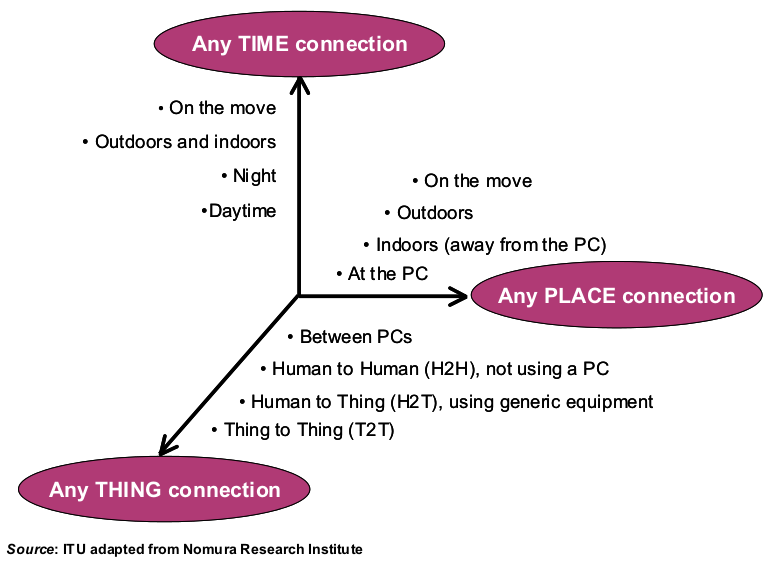
\includegraphics[scale=0.46]{images/12.png}
\caption{A new dimension}
\label{dimension}
\end{center}
\end{figure}

As the name suggest Internet of Thing is vision to connect all static items/things to web. To form a global network of \emph{things}, where they can communicate, and take decision by themselves. It mainly aims to develop our daily life more sophisticated and flexible. The phrase Internet of Things points out a vision of the machines of the future: in the nineteenth century, machines learned to \emph{do}; in the twentieth century, they learned to \emph{think}; and in the twenty-first century, they are learning to \emph{perceive}, they actually \emph{sense} and \emph{respond}. 

In the context of Internet of Things a ``thing" could be defined as a real/physical entity that exists and which is capable of being identified uniquely. Things are commonly identified either by assigned identification numbers (IDs) or names. In the IoT, `things' are expected to become active participants where they will interact and communicate among themselves and with the environment by exchanging data and sensed information about the environment. Things will also react autonomously to the real events. The possible outline of IoT future is shown in Figure \ref{roadmap}.

\vspace{0.5cm}
\begin{figure}[!h]
\begin{center}
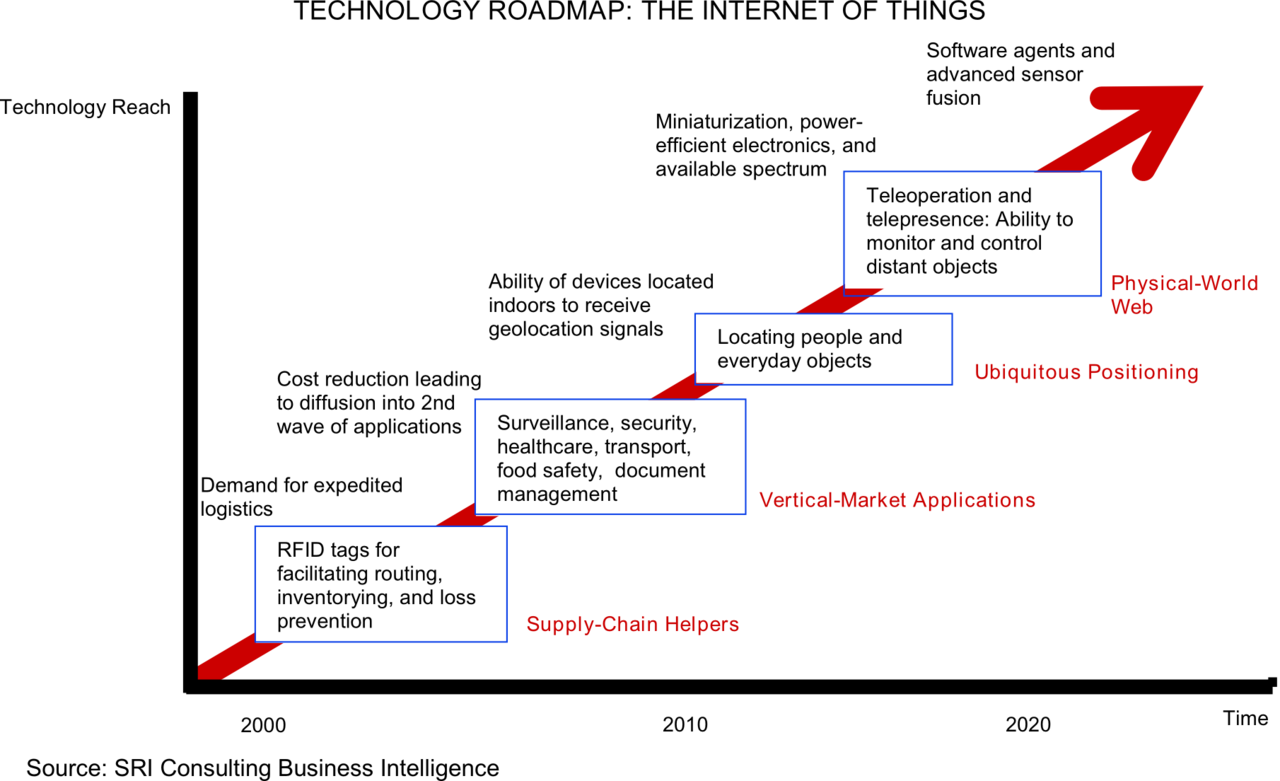
\includegraphics[scale=1.36]{images/1.png}
\caption{Technology Road-map : Internet of Things \cite{image_roadmap}}
\label{roadmap}
\end{center}
\end{figure}

It is a kind of smart objects' network which includes sensor, actuators and humans. This each object will have their own unique identity and each will have communication capabilities \cite{2}. Each object in this network consists of different types of sensor which collects the data from its environment and it either passes that data to other nodes or does some local processing on it. As Kevin Ashton said, \emph{``The Internet of Things has the potential to change the world, just as the Internet did. Maybe even more so.}"

\section{Intenet of Things: Technologies}
First in order to connect everyday objects we need a large global network, IoT uses Internet for this. Then to identify each object uniquely we need some mechanism. RFID offers this functionality. And lastly we need Wireless Sensor Networks to communicate between these smart items wirelessly (See Figure \ref{IoT:arch}). Initially IoT was proposed for supply-chain management where manufacturers can track their goods easily. As each item will be tagged, in future you will not have to stand in long queues for billing. It will be generated automatically using RFID reader at exit gates and tags attached to your purchased goods. 

\vspace{0.5cm}
\begin{figure}[h]
\begin{center}
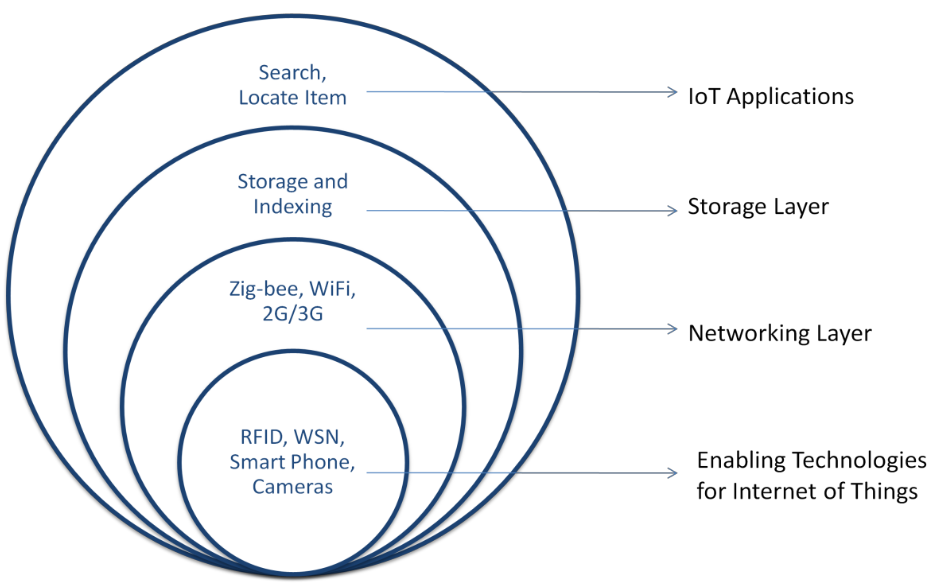
\includegraphics[scale=0.35]{images/7.png}
\caption{Internet of Things: Layer Hierarchy}
\label{IoT:arch}
\end{center}
\end{figure}

RFID uses radio waves to identify items, it is often seen as pivot enablers of IoT. It can be used to transfer data from an active or passive RFID tag to RFID reader wirelessly for the purpose of identification and tracking. Some early applications of RFID are like attaching a tag to every vehicle for automatic toll collection or a tag can be attached to every item during production to track its progress through assembly line. And now in Internet of Things vision these tags will be attached to almost each real world object including human!

Wireless Sensor Network (WSN) was mainly developed to monitor physical and environmental conditions like temperature, humid, sound, etc. The original motivation behind developing Wireless Sensor Network was military applications like surveillance. It is built of small `nodes' each of them has a transceiver to communicate, a micro controller to process locally, a circuit for interfacing various sensors and an energy source, usually a battery. In Internet of Things vision WSN is used to monitor a home or office, it is used to sense and pass the data to base station.

In case of IoT the networking layer uses Zig-bee, WiFi or 2G/3G cellular networks to communicate. Generally sensor nodes will use Zig-bee for short distance communications as motes have inbuilt transceivers for that.

The storage layer is for collecting all data at some central node. Like in case of WSN there is one base station which works as sink of network traffic. In IoT this database will be huge as there are millions of real-world items which will be tagged so to store and manage information about these all items we need some new storage and indexing approaches.

Last but not the least is the Applications, by which user will actually interact with the IoT. These can be finding any item in your home or getting a coffee ready when you wake up. This is the most interesting part of IoT, we will look at some more IoT applications in next chapter.

\section{Internet of Things: Application Scenario}

Alarm clocks go off early if there’s traffic on the way to office, plants communicate to the owners when it’s time for them to be watered, shoes communicate time, speed and distance so that their wearers can compete in real time with people on the other side of the world, medicine containers tell your family members if you forget to take the medicine! These are some applications which shows how our future life will be.

Consider another future scenario when you are living in smart home. You will not have to turn lights on/off by yourself, your home will automatically detect your presence/absence. It will prepare a coffee when you wake up, It will remind you to get an umbrella when it's going to rain outside. It will actually help you to find lost or misplaced items. Your home would also have fire and gas leakage detection that will take action accordingly in case of emergency. Not just home, this technology will change current transport services, warehouse management, precision agriculture, military and surveillance, etc. So we can say that our future life will be full of \emph{smart objects} which can \emph{sense, communicate} and \emph{take decision} by themselves. The Internet of Things will allow everyday objects to be identified, tracked, traced, and monitored. To give you more detailed idea about IoT see Figure \ref{cisco}.

\vspace{0.5cm}
\begin{figure}[!h]
\begin{center}
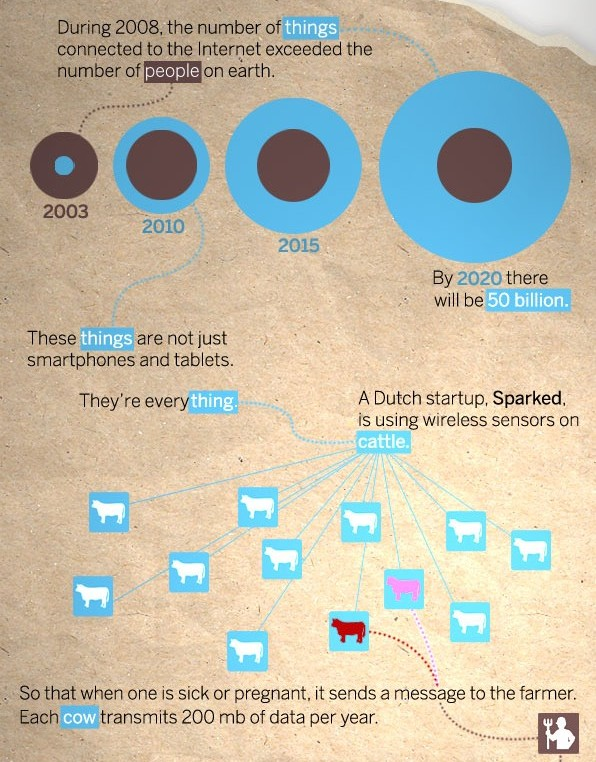
\includegraphics[scale=0.55]{images/2.png}
\caption{Internet of Things : Infographic \cite{image_cisco}}
\label{cisco}
\end{center}
\end{figure}

Some of the other interesting applications are as follow.
\begin{itemize}
\item Bicing \cite{3}, a public bicycle-sharing system in Barcelona, Spain, where users can see the number of bicycles available at each rental station in real-time on the web.
\item WEMO \cite{4} is another product which allows us to operate electronic appliances using motion control or a simple smart phone application.
\item Nike+iPod \cite{5} is a product in which you have to put a sensor in your shoe that will measure how much miles you ran. That sensor will also be connected to your phone through which you can track your progress daily.
\item Botanicalls\cite{6} is a system which allows plants in garden to texts/tweet their owner whenever they need water.
\end{itemize}

\section{Searching the Physical World: Motivation}

The most important objective of technology is to make people's life better. In this dissertation we propose a system to efficiently search any item in physical world in real-time. Today there are over 1.5 billion Internet enabled PC and over 1.0 billion cellphones which are connected to Internet. According to \cite{7} by 2015, we will have hundreds of billions of RFID – tagged objects connected to Internet that will generate lots of sensor readings every moment.

Now let's see why we would need new searching mechanism for physical world. As we have said IoT works in much larger information space than current Internet. We believe as document centric web, searching will become heart of IoT as well \cite{8}. Consider a common case when you are late for office and you could not find your keys! Our system will come to rescue in such situation which helps you to find out your keys. Searching is useful when you want to find a quite place for one day picnic. 

But there are some challenges while implementing a search technique. First a sensor network has to restrict the communication among nodes to  \emph{conserve power}. In Internet, servers have the web crawlers which would crawl web continuously looking for updates. In IoT it will not work as real-world entities are highly dynamic and sensor data changes rapidly. If we try to maintain a central database then updates will be very frequent and we need some novel data collection and storage techniques. Some other issues are like  \emph{scalability, real-time results, dynamic networks} and  \emph{security} concerns for user items. Some of the major challenges/issues for searching in IoT is defined below.

\subsection{Challenges and Research Gaps}
Now let's look at the things which makes \emph{Searching in Internet of Things} an active research area. What are the things that has to be handled differently then web search. Below we have classified five major challenges/issues/gaps that need to be handled while designing an efficient search mechanism.

\begin{itemize}
\item \textbf{Architecture Design}: In real world people do want to operate objects locally or remotely that distinguishes IoT search engines from commercial web search engines. And in case of wireless nodes the communication must be minimal to conserve power of nodes. Design requires new techniques ranging from crawling, indexing, storing and querying.
\item \textbf{Localized Search}: In case of IoT the mobile nodes are highly dynamic such that they can be part of network at any time and leave a network without prior notification. Unlike Internet where user wants to search remote database, in case of IoT user wants to search a thing or an item nearby to him like finding a key in his office.
\item \textbf{Scalability}: In IoT the environment is saturated with huge number of sensors, RFID-tagged objects. Sensors and RFID readers generate extremely huge number of readings which posses very short life span. So we need some novel storage and indexing techniques at server side to maintain such huge database.
\item \textbf{Dynamic Nature/Real-time updates}: This is one of the most important feature of IoT Search as user will require location of his keys instantly. For maintaining this real time data two communication paradigm exists \emph{timer} and \emph{beacon} scheme which can be regarded as push and pull based approaches.
\begin{itemize}
\item \emph{Timer Based} : In this approach the mobile node will send its own presence to central node. Once central node does not receives \emph{alive} message from a node within some period, it assumes that node has been moved to some other region. This approach is not energy efficient but more reliable.
\item \emph{Beacon Based} : In this approach the central node will keep broadcasting beacon frame periodically. And mobile nodes will reply to that only if it has changed its own position to mark their presence in new area. This techniques is energy efficient.
\end{itemize}
We also need some better data aggregation techniques to collect data at Basestaion.
\item \textbf{Privacy and Security}: As Ross Anderson pointed out that many security solutions will  fail when applied to different environments \cite{10}. Unlike the enterprise environment, where physical boundaries and firewalls can separate insiders and outsiders, users and service providers can coexists in a pervasive computing environments. Moreover the data content is also more important in case of IoT or Pervasive environments, as it might actually have users current location.
\end{itemize}

\section{System Overview}

In this section we will look briefly explain our system. As we already said, it can be used to find any real-world entity/item like your key/wallet/book etc. To start with, to find any item we must able to identify it first and then we have to find some approach to locate any item whenever user queries for one. 

To identify each item uniquely, we will tag each item which has a unique node id of it's own. To query for any item user has to enter it's node id in the GUI provided and our system will show where exactly the item is, with preloaded picture of that place. We have divided the whole space in various small localities. Each locality covers an area of about a table, so results will be shown upto that accuracy like {\em``Book is on study table of bedroom''}. We believe that it is often the way people organize the items.

For accomplishing this task we are using IRIS sensor motes for tagging and as mediators, a laptop/computer as base station which is network sink, where user can query and get results. The tags attached to real world entities will talk to mediators which covers area of bed/table. They again will talk to higher layer devices which represents room/office. And finally at the top they will communicate with base station which will handle all user interaction.

\subsection{Contributions}
Our main contributions are as follows:
\begin{itemize}
\item A data aggregation algorithm to collect data from large network at base station. This algorithm is being used to aggregate data. We will see this algorithm in detail in section 3.2.
\item A layered architecture to maintain hierarchy which helps to locate item easily. This layered architecture is insipred by the ways humans organize their things. We will look at the architecture in section 3.1.
\item And a hybrid approach to maintain location details of each item with minimum network traffic. We are taking advantages of both push and pull based approach to maintain location details. This approach will be descirbed in section 3.3.
\end{itemize}
We are also using hashing at server side for efficient memory utilization and faster access.

\section{Organization of the Thesis}
\begin{itemize}
\item In \textbf{Chapter 2} we will look at what is current research status and know about some of already implemented searching mechanisms. We will look at various searching schemes like object serach, place search, etc.
\item In \textbf{Chapter 3} we will propose our new searching mechanism and explain some of the algorithms of the system. In this chapter we will look at our system architecture first, a data aggregation algorithm, and a hybrid approach to maintain up-to-date data.
\item In \textbf{Chapter 4} we will explain how we implemented the whole system, using which tools, technologies and show some of the important functionalities of our system's various modules. We will also discuss some important test results at the end of this chapter.
\item And finally in \textbf{Chapter 5} we will conclude the thesis with possible future outline about how system can be extended.
\end{itemize}
In this chapter we described what Internet of Thing is and how it will affect everyone's life in future. We also looked at why we need searching mechanism and why current web search approaches can not be directly applied on IoT Search. In the next chapter we are going to look at related work done by research community in this area.

\newpage
\chapter{RELATED WORK}
\vspace{0.2cm}

In last chapter we have looked at what Internet of Things is, and how it will change our life. In this chapter we are going to look at the various work done till now. This chapter provides overview of existing searching techniques in IoT. We have classified the existing techniques in four different classes which are as follows:

\begin{itemize}
\item Components for IoT
\item Description Models for Connected Objects
\item Object Search
\item Place Search
\end{itemize}
Let's look at each of them in detail.

\section{Components for IoT}
This class of papers provides the idea about base technologies for IoT like Radio Frequency Identification (RFID) and Wireless Sensor Network (WSN).
 
A WSN\cite{20} is a collection of nodes which can sense and talk with each other. Each node consists of processing capability, may contain multiple types of memory (program, data and flash memories), have a RF transceiver, have a power source (e.g., batteries and solar cells), and accommodate various sensors and actuators to sense the surrounding environment. Such systems can revolutionize the way we live and work currently. WSN was mainly developed for military operations. In IoT WSN is used to communicate between \emph{smart things} and collect network data. It is also used to monitor and take decisions accordingly in smart home.

RFID is used to uniquely identify each item. It can be attached to item at time of production so that it can be tracked throughout it's life span. In future there will not be shortage or wastage of products as their owners would be able to track their products in real time and produce them according to market needs.

SixthSense\cite{21} describes about how to tag each real-world item and how to identify which tag belongs to whom or what. It uses various heuristics for this like tags attached to people are more likely to move with less dependence on other tags, than tags attached to objects. Similarly, the owner of the object is likely to be the person who carries it around most of time.

SixthSense also uses information from calendar, or login information to detect user presence. In this way system first infers range of information based on accumulations of observations and provides some basic applications like lost object alert, enhanced calendar, etc. It also provides a set of APIs to build an application on top of it which contains methods like, GetTagOwner(TagID) or GetOwnedObjects(PersonTagID), etc.

\section{Description Models for Connected Objects}
This class of paper focuses on finding proper web resource description that enables both humans and machines, to semantically discover functionality provided by Web-enabled device. This will lead to finding, selecting and utilizing smart things. The task of finding relevant smart things is more complicated than web search because of dynamic nature, real-time updates, and absence of uniform way to describe things.

Searching WoT\cite{22} focuses on these three main areas: (i) Defining description model for connected objects (ii) Clustering similar connected objects and (iii) Searching. First system describes the objects in semantic models like its capabilities, its location, etc. After describing each object it tries to cluster them according to their capabilities or according to their input they take. And in search part authors proposes on going work in which they try to identify who is the requester a machine which needs quick results or a human who needs accurate results.

Search Engine Framework\cite{23} presents layered architecture consisting of ``sensor monitoring layer",``storage layer", and ``index layer". The lowest layer components monitors real-world environment continuously. While storage layer stores data in terms of “monitored object”, that is all sampling values of same object are organized together within same record. And at index layer various indexing techniques have been used which can provide fast access to data records stored at storage layer.

In summary, all of these papers focuses mainly on how to represent the smart object or how to store them in database so that user can get accurate information faster. Searching WoT defines different semantic models, interlinked through properties to describe an object and then it clusters them together, while Search engine framework defines various indexing schemes for storing the data.

\section{Object Search}
This class refers to the methods to implemented about finding any misplaced item in pervasive environment where each real world entity would have been tagged. Here we are surveying six different methods to do so.

The basic technique behind Snoogle\cite{11}\cite{12}, MAX\cite{13} and OCH\cite{14} is similar and it is as follow:
\begin{itemize}

\item In Snoogle and MAX a sensor node is attached to each real world object and it carries textual description of that object in form of keywords, user can query system using these keywords. While in OCH each object stores unique identifier for each object instead of textual description.

\item This textual description can be anything like for a novel it might be ``Book: The Immortals of Meluha, Author: Amish". So now whenever user queries for any of this words weather it is the title or author's name, this book will be shown in the results presented to user. So for better accuracy these systems assumes end-user has to tag each item sensibly.

\item In terms of architecture, Snoogle and MAX both adopts similar hierarchical structure.
\begin{itemize}
\item In Snoogle (See Figure \ref{snoogle}), the top most level is KeyIP (Key Index Point) which can be more than one in network and that works as sink. The KeyIP collects data from different IPs and holds the global object aggregation information. It is assumed to have constant power supply and powerful processing capacity.

\vspace{0.5cm}
\begin{figure}[!h]
\begin{center}
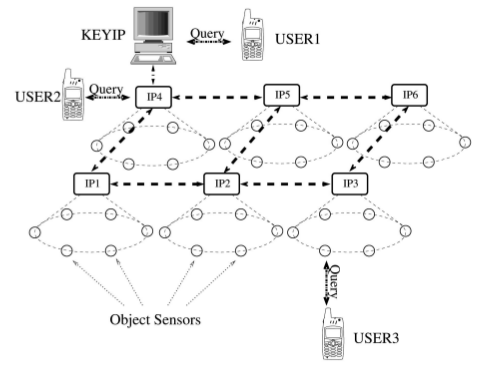
\includegraphics[scale=.6]{images/3.png}
\caption{Snoogle Architecture \cite{11}}
\label{snoogle}
\end{center}
\end{figure}


\item Just next to it, there are IPs (Index Points), it is a static sensor device which is associated with a physical location. IPs are responsible for collecting and maintaining data from object sensors in their vicinity. They build the inverted index of items for performing a local search.
\item In lowest layer, there is Object Sensors which are attached to real-world entities. They can be stationary or moving. Snoogle assumes that sensor data is already preloaded or incrementally added by owner.

\item In case of MAX (See Figure \ref{max}) objects at each level are more mobile than objects in higher levels. Tags are at the lowest layer and are attached to physical objects which are easily movable. These tags have to extremely cheap and small in order to use widely. They are assumed to have either limited or no power supply. Given this conditions RFID tags are the most suited options.

\vspace{0.5cm}
\begin{figure}[!h]
\begin{center}
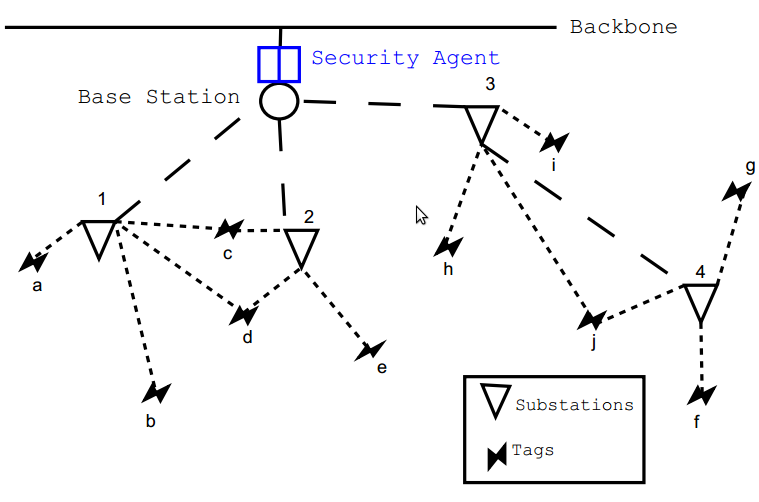
\includegraphics[scale=.4]{images/4.png}
\caption{MAX Architecture \cite{13}}
\label{max}
\end{center}
\end{figure}

\item Just above the tags, there are sub-stations. Sub-stations are powered by batteries, they also store label or description of the object they are attached to. Sub stations represents the entities which are relatively static like study table, cupboard, etc. Sub stations have dual role, first they have to act as RFID readers too query rags in their range. Secondly, they have to forward results to base station.

\item Base stations are at the highest level of hierarchy, and represents the immovable locality such as room or office. These base stations also works as mediators between wired backbone network and wireless tags.
\end{itemize}

\item OCH uses Bluetooth for prototyping; it uses Bluetooth enabled mobile phones as object sensors which detects the presence or absence of tagged objects.

\item The main issue handled by OCH is that in OCH queries are not sent to all object sensors for scalability reasons. Instead of broadcasting this system uses probabilistic measures and various heuristics like
\begin{itemize}
\item Lost object might be at the place where owner spends most of the time
\item It might near to a location that owner has visited recently 
\item Near the location where object was last see
\end{itemize}

\item End user can associate various priorities with any of the above heuristics. In general the query contains identity of the object required, above priorities, timeout t and budget q.

\item These both approaches Snoogle and MAX are unable to scale well as Snoogle uses centralized approach to store indices and in MAX each query has to be sent to each tag.

\item In terms of privacy Snoogle uses UNIX like access permission attached with items and MAX assigns each node as either private or public.

\item Distributed Image Search (DIS)\cite{15} uses camera as sensors. Users can pose a queries by specifying an image and the system returns details of sensors that have captured similar images. Then results are ranked and only top-k results are returned to user. To avoid transmitting whole image this system uses a feature extraction mechanism that maps an image to set of visterms (similar to keywords) to describe th image. After capturing an image a sensor node converts it to visterm. And this resulted visterms are stored in inverted index for efficient lookup.

\end{itemize}
Other techniques like AURA\cite{18} and SCPS\cite{19} can also be used to guide user to find a misplaced item but using different approach than above. 
\begin{itemize}
\item Without requiring periodic location updates, SCPS locates user objects based on their routine movement pattern. It also uses social-aware Bayesian networks to predict user location in exceptional cases like rain or illness which breaks routine pattern. It generates distributed search based on DHT (Distributed Hash Tables). 

\item This system uses hierarchical structure with Base Stations on upper layer and Mobile Nodes and Sensors on lower layer. Whenever a request comes for an object, first owner of that object is found and then based on owner's pattern and Bayesian network his current location is found.

\item AURA uses novel approach to enrich the physical environment with information about objects to facilitate search. It uses environmental RFID tags to store data about smart-object's location as distributed storage cloud. It uses EPC GEN 2 RFID protocol to write data to passive RFID tags which works as short term memory for user activities and object interactions. 

\item This system proposes two algorithms \emph{auraProp} to disseminate information in environment and \emph{auraSearch} to find an physical item in real world. And each user keeps an interrogator device which will pick up information about objects in its current vicinity and spreads this information along the path user follows (leaves aura). User also needs some kind of RFID reader or PDA with him to make an query which contacts its environmental tags and finds out location of required item based on stored data on them.
\end{itemize}

In summary this all algorithms help user to find an item in smart world. Snoogle, MAX, AURA and OCH assumes to tag each real-world, and SCPS help to find an item belonging to user at a time. Snoogle and MAX stores the textual description of the item while OCH stores the identifier on tag. Snoogle, MAX and OCH are kind of centralized approach while AURA uses distributed approach in which environmental tags are used as storage cloud.

\section{Place Search}
This class of papers mainly focuses on finding a place or location according to user's preference. 
Suppose you want to go and relax for a day, then you can query the system with parameters like less crowded and near to home. Or in the office you might want to find an empty room for an urgent meeting. This section provides information about various such systems.

In Dyser\cite{17} each sensor and entity has a web page where it keeps publishing latest data. The UI design is similar to web search like 'Italian Restaurant:quite'. In this query there are two parts, one 'Italian Restaurant' is sought using static entity page and the term 'quite' will be searched using sensor page for loudness sensor. Dyser consists of a resolver, index and an indexer. Index stores meta data on sensors and entities, while indexer keeps crawling sensor and entity pages. 

Dyser also uses various prediction models which returns the probability of a sensor reading a specific value at given time. Whenever user queries for something, system first ranks the sensors in order of their probability of delivering desired result, and then system starts querying the sensor with highest probability. In this way system does not have to contact each and every sensor for a query, which makes Dyser more scalable. Dyser uses two different ranking schemes one for which sensors to be considered and another for user's preference.

Sensor Similarity Search is not a keyword based search engine like previous approaches, it uses search-by-example technique. According to authors in real-life different person uses different terms to describe same concept. So different users use different keywords to describe a sensor which effectively does the same thing.And this problem can be related to multimedia search like image and video search which uses search-by-example technique. 

Authors proposes, a method where given a sensor, other sensors on IoT are found that produced same output patterns in past. System uses fuzzy logic to compute the similarity score among pair of sensors. It also uses sensor gateways to crawl through sensor output periodically. All sensors computes the fuzzy set which represents its past output. These sets are then indexed at central database. And finally at time of query a similarity score for each indexed sensor is calculated.

This service could be used in different ways, suppose one wants to find a place that have similar physical properties. For example if one wants to find a place which has same climate as a known place A, he could pick temperature sensor of place A and search for other temperature sensor with similar output.

So in summery these algorithms provides methods to find a location covered by sensors according to user's need. Dyser uses prediction, indexing, and ranking scheme to efficiently find a location and sensor similarity search provides search-by-example interface and uses fuzzy logic to compute final results.

Apart form these all classes we have also covered various survey papaers as part of our literature survey. Survey papers are great to get an overall idea of whole concept. The papers which have been covered talks about various other methods implemented for searching and also provide some common challenges in this area.

Authors of ``Internet of Things: Vision and Challenges" \cite{9} talks an idea about origin of Internet of Things, and then defines some challenging issue of searching. While authors of ``Real-time Search for Real-world Entities: A survey" \cite{16} describes overview of each searching method and authors propose their own search engine in the end. ``Where Searching Will Go" \cite{24} defines some basic characteristics of IoT and provides challenges and then authors present their ongoing work about a search engine.

In this chapter we have looked at various already implemented methods for item/place search. We also covered various methods which are used to define how we should describe each item and how to assign semantic meanings to them. In the next chapter we will propose a new searching technique which will try to overcome the problems faced by this systems.

\newpage
\chapter{PROPOSED WORK}
\vspace{0.2cm}

In this chapter we will propose some new approaches to tackle the problems defined in section 1.5. We propose a new hierarchical architecture which will improve the scalability of the system and will generate results in real time. We are also considering search locality as our results will find an item locally. Then we will describe our data aggregation algorithm which is used to collect data at base station. Next we will discuss our novel approach to maintain up-to-date data in through hybrid combination of push and pull communication paradigm. At last we will show the overall working of the system and how it works.

\section{System Architecture}

An idle architecture is the one which is easy to setup and configure with existing environment. Our this architecture is inspired by MAX\cite{13}, in which authors argue that the main motivation behind such hierarchical architecture is the way how humans organize his/her things. Generally to locate any item, people will first provide in which room it is (provided by mediator layer 2), followed by identifiable landmark like table or shelf (provided by mediator layer 1). 

As shown in Figure \ref{system:arch}, we are adopting a hierarchical architecture made up of four layers. Lowest layer entities are the \emph{tags}, items which moves most frequently (e.g. keys, wallet, cell phone), in most of the cases user will be interested in finding one of these items. Just above it, there are \emph{mediator level 1}, which represents entities which are moved occasionally and less frequently (e.g. table). Next to layer 3 there are \emph{mediators level 2}, entities that are immovable (e.g. room/office) and Layer 1 is the Base station which is sink of network.

In our system we assume that each item will be tagged and will contain some unique id to it. Once each item is tagged by user, there no further maintenance he/she would have to perform except changing batteries. Now let's look at each modules of the system in detail. The system architecture is shown in Figure \ref{system:arch}.

\vspace{0.5cm}
\begin{figure}[!h]
\vspace{0.5cm}
\begin{center}
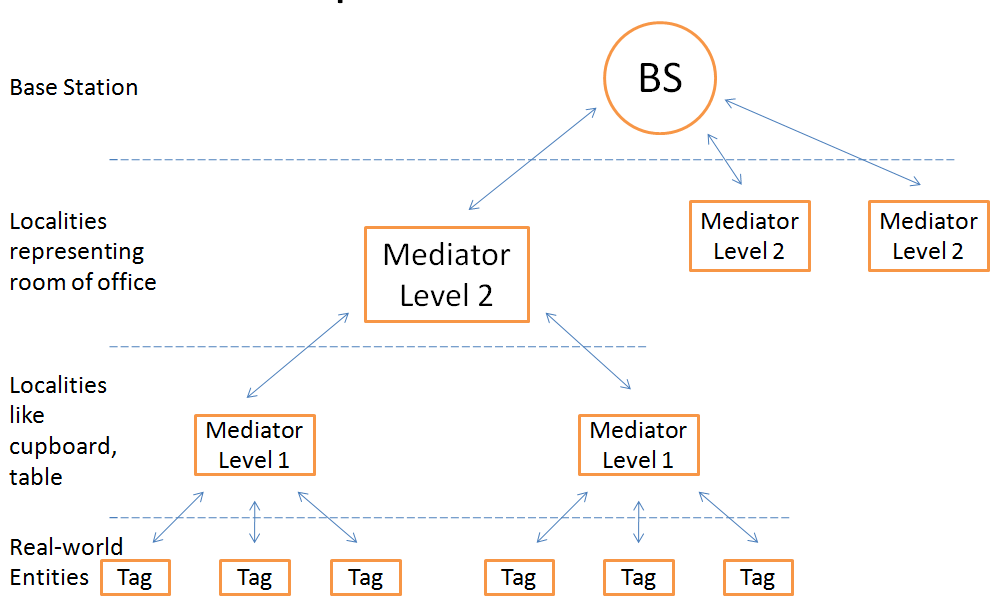
\includegraphics[scale=0.65]{images/8.png}
\caption{System Architecture}
\label{system:arch}
\end{center}
\end{figure}

\begin{itemize}

\item \textbf{Base station}: Base station is at top most layer in hierarchy. In our system there is single base station which is considered to have constant power supply. User can post query to find any item and see results at base station. As we will see below we have divided each item in two different categories namely push and pull. Base station will store details and current location about push tags. We are using hashing to store the locations as it provides various benifits over arrays, like faster time access and efficient memory utilization.

\item \textbf{Mediator Level 2}: These layer 2 devices covers area approximate of a room or office. It represents immovable entities. These device have mainly two tasks, one is to pass data from mediator level 1 to base station and user queries from base station to lower layers. Second is to forward data to base station using the data aggregation protocol defined below. 

\item \textbf{Mediator Level 1}: Layer 1 mediator covers area like a table or bed or cupboard. These device will take care of the tags present in its region and pass that data to upper layer that is Mediator Level 2. For push tags this mediator will make an array of items under its region and pass it to upper layer at specific intervals. Major tasks of this layer is to pass data from tags to upper layer and user query from upper layer to the tags. For implementation purpose we have used IRIS motes to perform this task.

\item \textbf{Tags}: In our system each real-world entity will be tagged. For now we are using IRIS motes to tag items. This tags just stores their unique node id in them by which end-user will search for them. These tags are lowest layer items which represents various \emph{things} like shoe, book, cloth, etc. This are the items which moves most frequently in one's home. In general user will usually query for one of these items. So now for a user to be able to find out these items we have to maintain a database at base station to store their locations. But doing so will generate a huge database at Base station so to cope up with that we have divided these items in two different categories.

\begin{itemize}
\item \emph{Push Tags}: These are the items which will keep broadcasting their locations periodically. Base station will keep track of these tags and store their locations in its local database. So whenever user queries for one of these item base station will reply directly from local database. We will attach these tags to the items which are required in emergency like medical kit, fire extinguisher. Items which needed immediately and misplaced frequently like keys, wallet will also use this push tags so that it can be sought instantly.

\item \emph{Pull Tags}: These are the items which are relatively more static than previous one. These tags will only transmit their location when user queries for that particular item. They will not periodically broadcast anything. Items in this category can be books, cloths, etc. Which are not needed immediately and which moves less frequently. So whenever user queries for one of these items the Basestaion will broadcast that query and one particular tag will reply to it.
\end{itemize}

\end{itemize}

\section{Data Aggregation Algorithm}

As we are proposing a methodology to find any item throughout your home. It might be the case that some mediator's data can not reach to base station directly because it is far away from its range. Like if we have setup base station in one of the bed rooms, then clearly mediators of drawing room can not pass data to them directly. In such cases, we must have some kind of multi-hop protocol to pass and aggregate data at BS. In this section we propose a new data aggregation algorithm to collect all data in the network at basestation. Generally the periodic updates from push tags will use this algorithm to inform BS about their current locations.

We are assuming base station will be having node id: 0.
\begin{figure}[!h]
\begin{center}
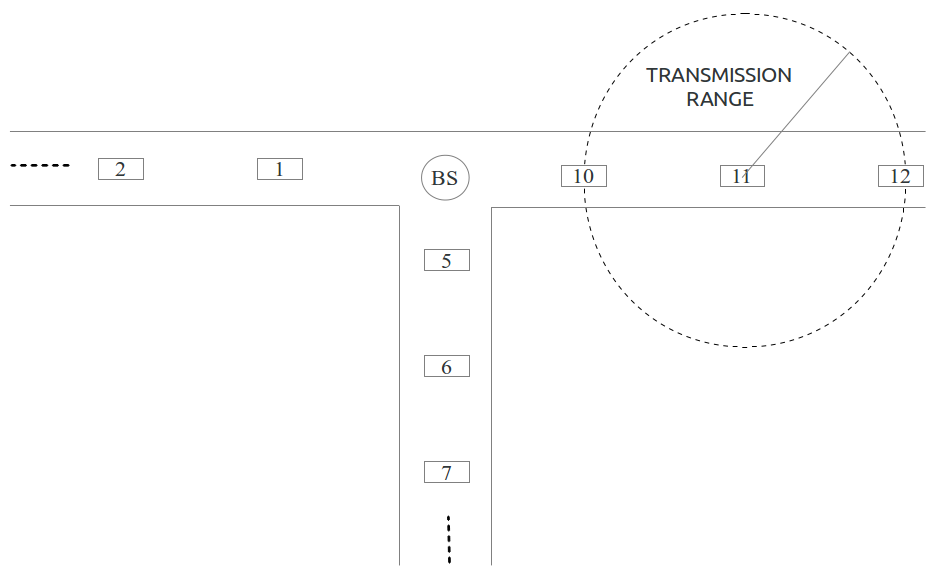
\includegraphics[scale=0.47]{images/9.png}
\caption{Data Aggregation}
\label{aggregation}
\end{center}
\end{figure}

To make things more clear, consider a scenario shown in Figure \ref{aggregation}. Here each box represents a locality similar to a room so each of boxes represents a mediator layer 2 entity, and number on them is their node id. Now as one can see Basestation(BS) is at center of building and so it is not possible for each mediator to pass data to BS directly and we have to use multi hop algorithm. Like node 11 can transmit only to node 10 and 12 with its range, so our algorithm is useful when it wants to pass some data to base station.

Our main assumption for algorithm to work is that mediator node ids will keep decreasing as we proceed near to base station. So we can say if a packet wants to reach to base station than it must go in direction of lower numbered nodes. Suppose if node 7 wants to send some data to BS then it can not do it directly, it will pass that packet to 6 which will pass it to 5 and finally 5 will pass that packet to BS.


typedef nx\_struct AggregationMsg

\{

  \hspace{2em}nx\_uint16\_t nodeid;\hspace*{3em}	\emph{Mediator node id.}

  \hspace{2em}nx\_uint16\_t size;\hspace*{4em}	\emph{Number of nodes under that mediator.}

  \hspace{2em}nx\_uint16\_t nodes[10];\hspace*{2em}	\emph{Node ids of the items}

\} AggregationMsg;


Above is the paceket structure that will bt passed by this data aggregation algorithm. Let's look at Data Aggregation Algorithm:
\begin{framed}
\begin{enumerate}[1.]
\item \textit{Wait for aggregation packet.}
\item \textit{Retrive source id of packet received}
\item \textit{If (source\_id $>$ own\_node\_id)}

\hspace*{2em} \textit{forward it}

\textit{else}

\hspace*{2em} \textit{do nothing}
\item \textit{Go to Step 1.}
\end{enumerate}
\end{framed}

As we have already said this algorithm will be implemented by each mediator which is used to collect information about push tags. Now consider an example when node id 11 want to send a packet to basestation as shown.
\begin{enumerate}
\item Node 11 will generate a packet and broadcast it.
\item Node 12 and 10 both would receive it and they will check to condition defined in algorithm step 3.
\item Condition will be true for node 10 and it will forward it while node 12 will just discard it.
\item So now when node 10 will forward it, packet will reach to it's destination i.e. base station.
\end{enumerate}
In this way the data will finally aggregate at basestation from the whole network through multiple hops transfer. We are also using similar approach for broadcasting user queries to each tag and getting replies from far away mediator in case of pull tag search.

\section{Push-Pull Based Hybrid Approach}

Now as we have said we need a mechanism to know exactly where user requested item currently is. There are two ways to do that, (i) store location about each item and reply whenever user queries for something, (ii) whenever user queries for some item search for it. For maintaining up-to-date data about item locations, two communication paradigms exists. Let's look at both of them in detail.

\vspace{0.5cm}
\begin{figure}[!h]
\centering
\mbox{\subfigure{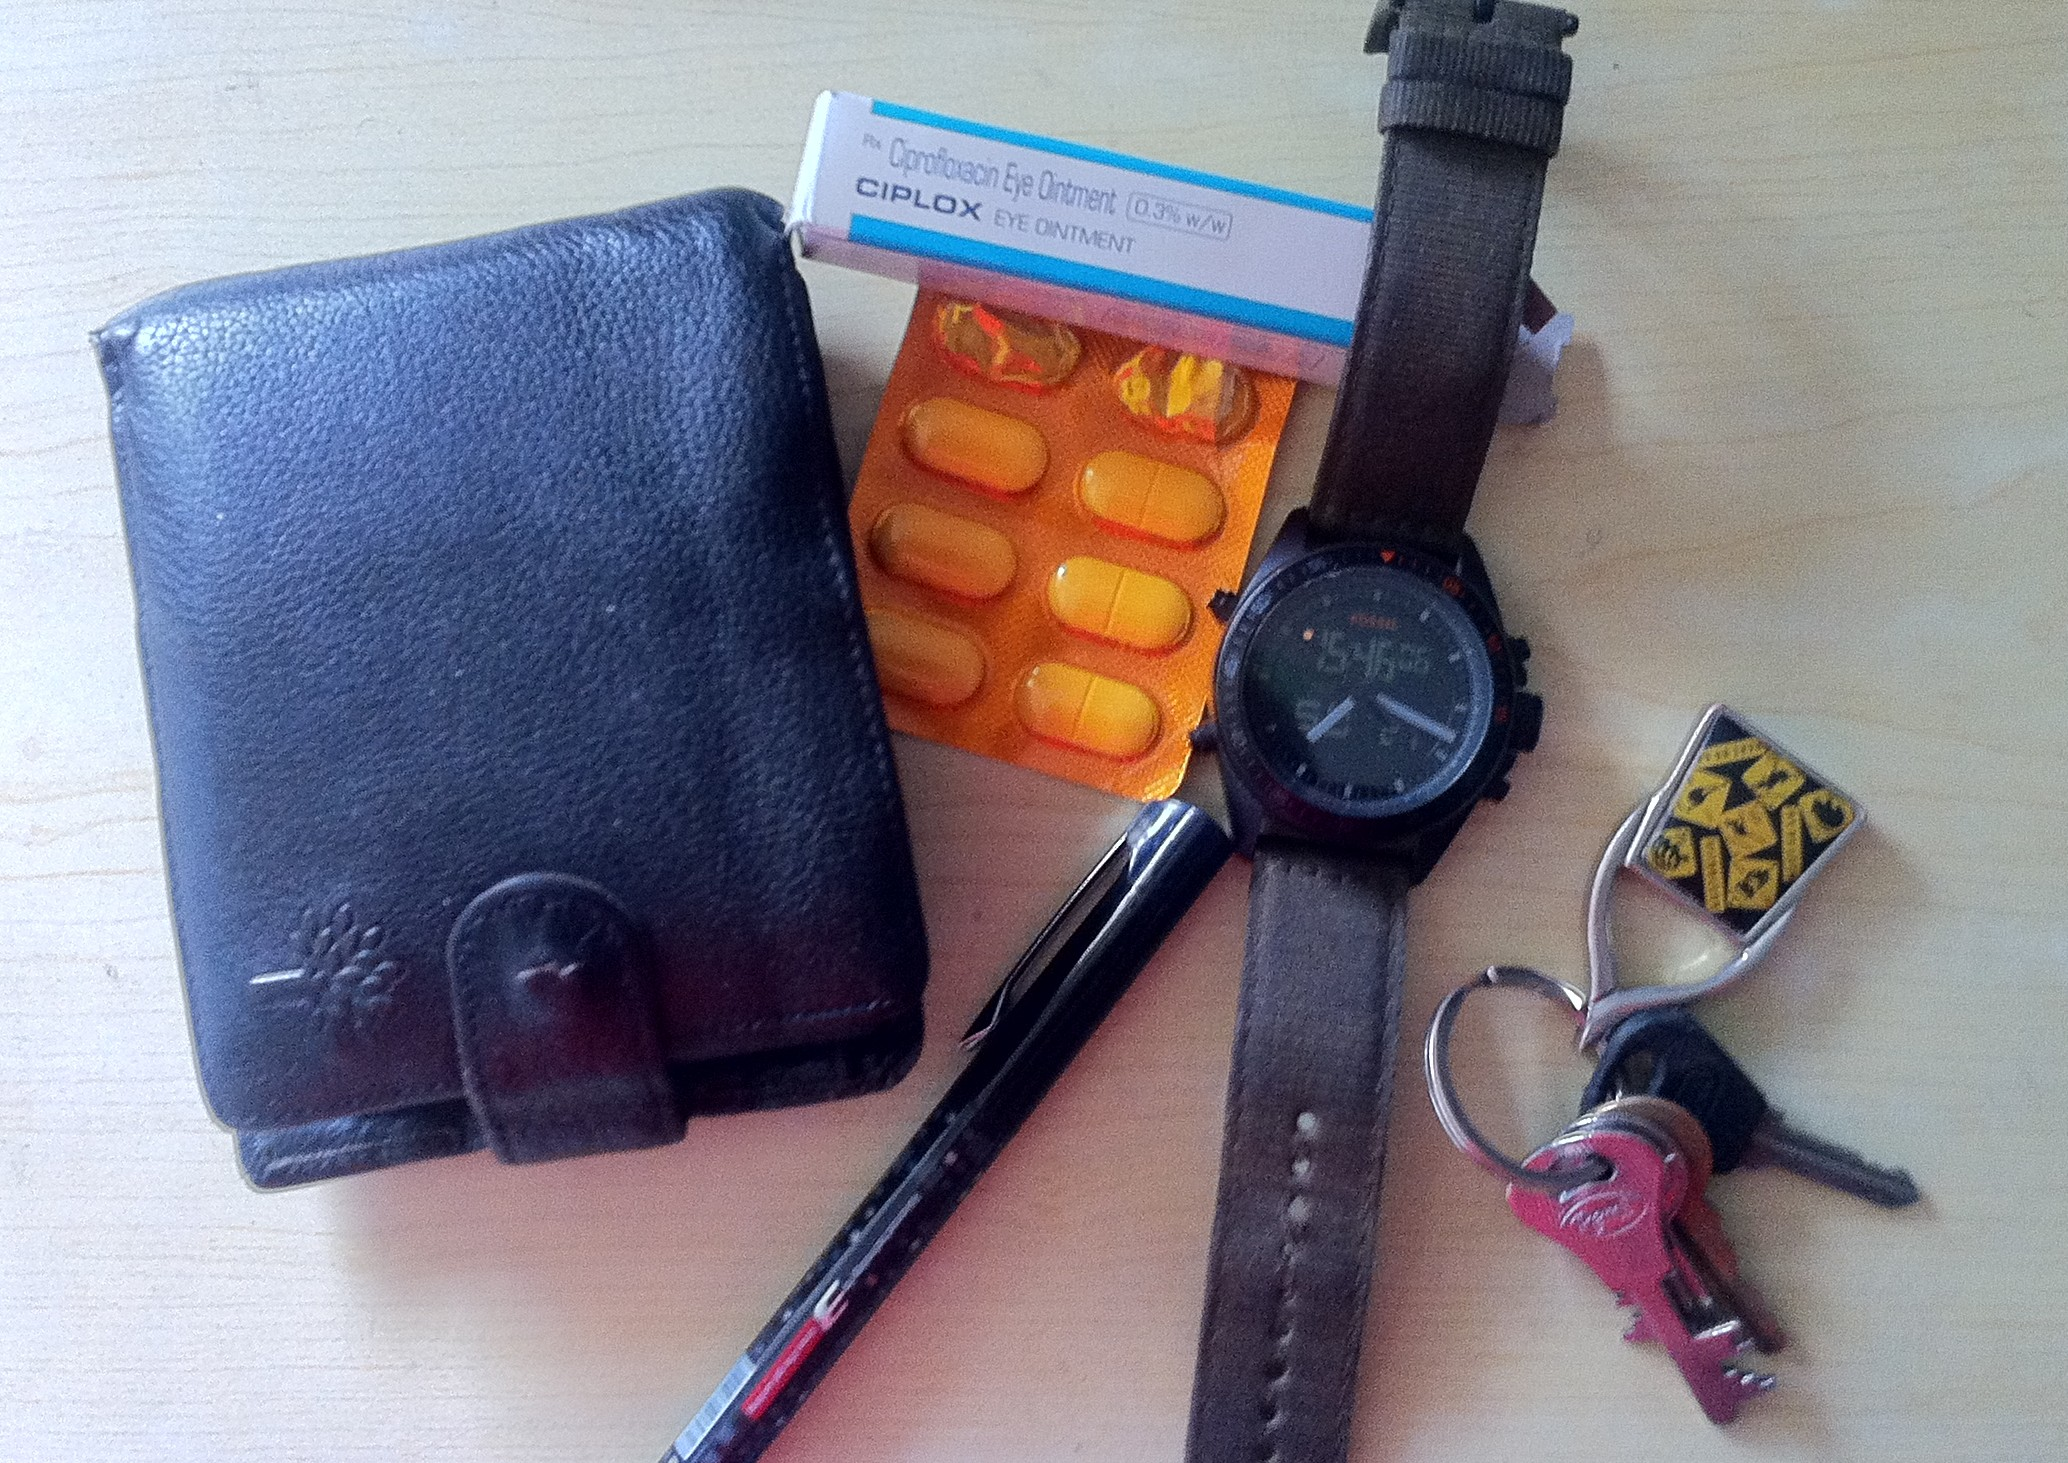
\includegraphics[scale=0.1]{images/13.JPG}}\quad
\subfigure{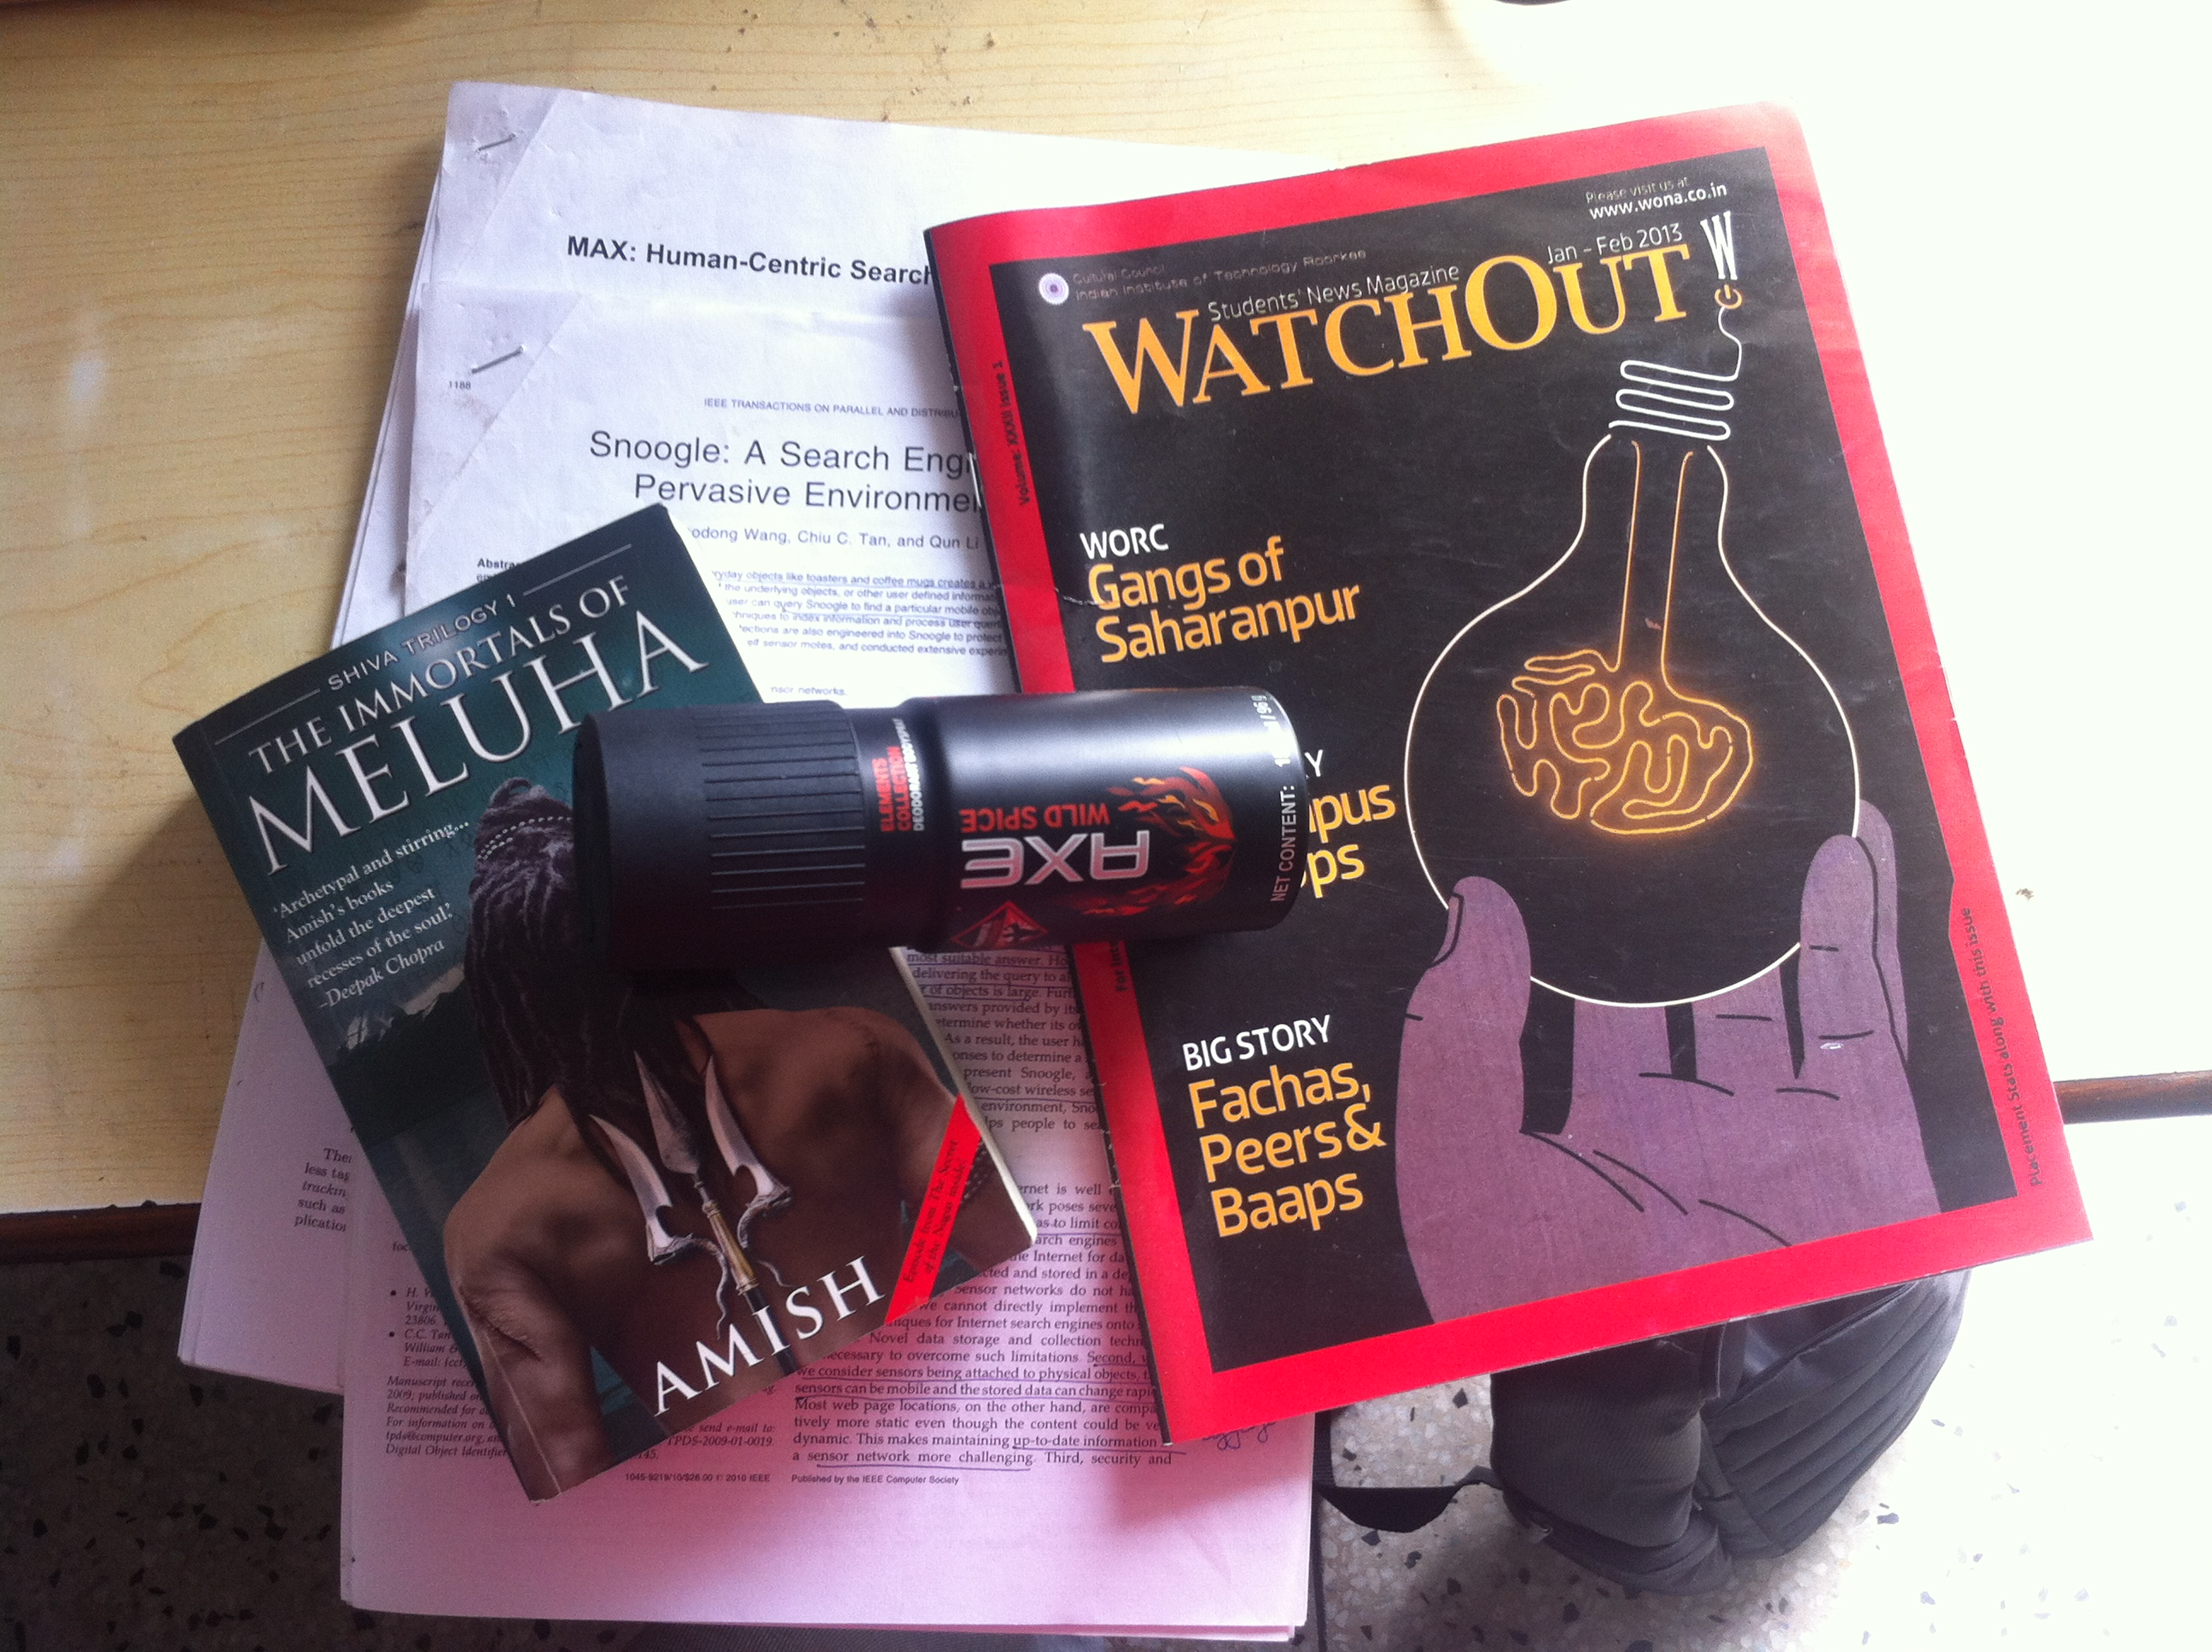
\includegraphics[scale=0.075]{images/14.JPG}}}
\caption{Push and Pull Items: Example} \label{hybrid}
\end{figure}

\begin{itemize}
\item \textbf{Push Based:} In push approach each item keeps \emph{pushing} their details to upper layer. And that pushed data is finally aggregated at central node. Once aggregation node does not receives any message from particular tag it will assume that it has been moved out of range. This approach guarantees up-to-date information but is not an energy efficient as nodes will have to publish their details periodically. 

\hspace{1em} In our system tags will broadcast their presence periodically which will be passed to mediator level 1 to mediators of level 2 and finally it will reach to base station using data aggregation algorithm defined above. As we know there are lots or items/things in home so information about these items creates huge traffic in network as well as large database at basestation. Even maintaining this large database is hard as updates will be too frequent because of frequent item movements. This technique will generate results instantly as base station will have information about all nodes in network. But as we have said it is not energy efficient as each node will have to broadcast their presence periodically.

\item \textbf{Pull Based:} In pull based approach, items will not have to transmit anything. In fact they won't have to do anything till user requests for any item. Here base station will send query to each node when user queries for anything. In a way user has to \emph{pull} item's current location. 

\hspace{1em} In pull based approach there will be no central database. Whenever a query comes to base station it will be forward it to mediators of level 2, they will pass it to mediator level 1 which will check for quired item in their regions. And finally they will report presence of quired item to basestation. This technique is energy efficient as well as network friendly because tags do not have to transmit anything at specified time intervals. But this technique is slower compared to push approach, because at time of each query it has to be broadcasted and user has to wait till it reaches to all tags and one of them replies. Table \ref{comparision} shows advantages and disadvantages of both approaches.
\end{itemize}

\begin{table}[h]
\newcolumntype{L}{>{\centering\arraybackslash}m{4cm}}
\centering
\caption{Comparison between Push and Pull Approach}
\vspace{0.2cm}
\label{comparision}
\begin{tabular}{|L|L|L|}
\hline
Communication Paradigm & Advantages & Disadvantages \\ \hline
Push Based Approach & Faster search, Instant results & High network traffic, huge database, energy inefficient \\ \hline
Pull Based Approach & Energy efficient, Less network traffic & Relatively slow response \\ \hline
\end{tabular}
\end{table}

As we can see, there are pros and cons of both, so instead of using single approach we will use hybrid mechanism to maintain uptodate data. What we propose is that we will use push based approach for the items which are important or might be required in urgency or lost frequently. See figure \ref{hybrid}, the items on left are the once which uses push approach to maintain up-to-date data. Things like first-aid kit, medicines which you need in case of emergence or wallet, keys, etc. which you always find at time of leaving home. This all items will keep pushing their location to basestation so at time to query we will get result immediately. By using this approach there will not be problem of high network traffic or database maintenance because count of these items will be limited. We can roughly approximate 50-100 such items in one's home and maintain g information about them is relatively easy.

While for other items like books, cloths, magazines (See Figure \ref{hybrid}), we will use pull based approach as we do not need them instantly. User can wait for some seconds while querying these items. These are the items which are relatively static compared to previous one.

We can say our approach is better than using push only or pull only approaches. As in our approach, there will not be too much traffic in network as only some items will use push based approach. Which makes database maintenance at server easier. And it will also produce results faster for the items which are required urgently.

\section{System Operation}
In this section we will look at how our system works, how user can query for item and get the results. Figure \ref{gui} shows the starting screen of our system, through which user can query. 

\vspace{0.5cm}
\begin{figure}[!h]
\begin{center}
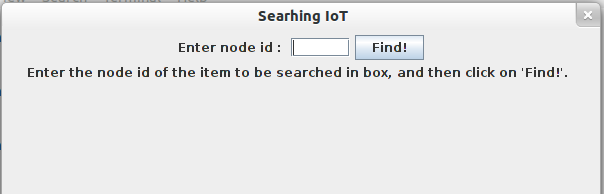
\includegraphics[scale=0.7]{images/15.png}
\caption{System GUI}
\label{gui}
\end{center}
\end{figure}
immediately
User has to enter the node id of an item to be sought in box provided and click on \emph{Find!} button. Just after pressing that button our system tries to recognize which class that sought item belongs to i.e. {\em push} or \emph{pull}. According to class one of following methods will be executed.

\begin{enumerate}[1.]
\item In case of push item, our system will look at local database entry for that item and show it's location to user immediately. Because if it a push item, the item would keep pushing it's details to BS and base station would have most latest location.
\item In case of pull item, user has to wait for some time. System will prepare a user request packet and broadcast it to all mediators which will forward request to tags. These tags will compare their own node id to requested id, and reply if user is looking for them. Once this reply packet reaches to base station, it displays location of sought item to user.
\end{enumerate}

Using one the ways our base station finally gets the results and shows it to end user (See Figure \ref{result}).

\vspace{0.5cm}
\begin{figure}[!h]
\begin{center}
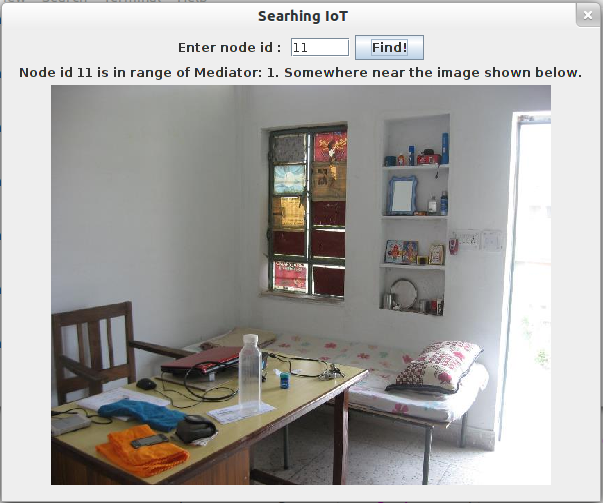
\includegraphics[scale=0.7]{images/16.png}
\caption{Results: System showing item's current location}
\label{result}
\end{center}
\end{figure}

In this section we have looked at the main part of this thesis, the design of our searching algorithm. During the whole system design we have tried to overcome all the issues/challanges dicussed in section 1.5. 
\begin{itemize}
\item As we defined we are proposing a new architecture for efficient search and to overcome power limitations, we are using pull appimmediatelyroach for most of the item which saves energy. 
\item To overcome scalability we are using hybrid approach, that reduces the network traffic as well as frequest database updates and which also delivers quick results for some items.
\item Again for the problem of real-time updates, the hybrid approach works fine as there will small number of items which will use push based approach.
\item And to overcome problem of localized search we have divided the whole physical space in mediators which covers small areas. Once we give user an approximate location, he/she can easuly find out an item.
\end{itemize}

In this chapter we have given the details about our work and proposed system. We have discuused about layred system architecture, an data aggregation algorithm to collect data at base station from a large network, and a hybrid push-pull apporach to efficiently maintain up-to-date data about various items. In the next chapter we will look at which tools and technologies, we have used to implement this work. We will also look at the workings of push/pull tags, mediators and of base station in more details.

\newpage
\chapter{IMPLEMENTATION AND TESTING}
\vspace{0.2cm}
In last chapter we have looked at our proposed work, system architecture, and some algorithms. In this chapter we will discuss about how we implemented them. We will first look at which hardware tools and software technologies have been used to implement them, and after that we will look at the working of each module in detail. And in the last we will show some important results.

In our system, we have used IRIS motes as mediators and same for tagging real-world entities. Because of transmission range of IRIS motes can not be reduced up to range of one table or bed we have eliminated mediators of level 1 from the implementation part. Tags will directly contact layer 2 mediators which will pass that data to BS.

For implementation of tags, mediators and base station we have used \emph{nesC: A TinyOS programming language} for programming the sensor motes. And for base station we have used \emph{Java} to design overall GUI of the system.

\section{Tools and Technologies}
In this section we will look at various hardware tools and software technologies used to implement our system. We will first start witht the hardware modules and continue with software technologies.
\subsection{IRIS Motes}
IRIS (see figure \ref{iris}) is 2.4GHz mote module used for enabling low-power, wireless sensor network.

\vspace{0.5cm}
\begin{figure}[!h]
\begin{center}
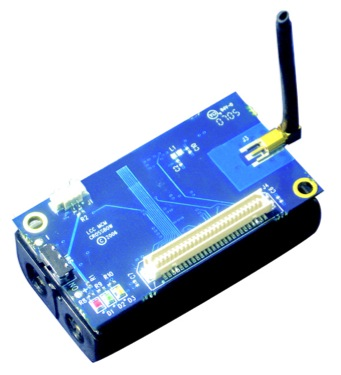
\includegraphics[scale=0.45]{images/17.jpg}
\caption{IRIS mote}
\label{iris}
\end{center}
\end{figure}

It has IEEE 802.15.4/Zig-bee compliant RF transceivers for wireless communication. The transmission can speed upto 250 kbps. The data can be sent and received through walls and no line-of-sight is required for two motes to exchange data. It has 8KB of RAM, 128KB of flash memory and an ATmega 1281 low-power micro controller for commutation purpose.

These motes are designed specifically for deeply embedded sensor networks. Each node can work as router for wireless communication. Various other sensor boards for sensing light, temperature, RH, pressure, etc can be attached with mote. The IRIS 51-pin expansion connector supports analog inputs, Digital I/O, I2C, SPI and UART interfaces.

These motes run an operating system specifically designed for low-power devices, \emph{TinyOS}. And the language used to develop that OS is \emph{nesC}, same language is used to even program this motes. In our system we have used these motes as mediators as well as tags. We just upload one of the two program and same mote can work as either of them.

\subsection{Mote Interface Board}
As we have discussed in our architecture we have one base station in our network which works as sink. This interface board is used for that purpose, it provides USB connectivity to motes. Any MICA/MICAz/IRIS mote can work as base station when it is programmed in such way and is attached to one of this boards (see figure \ref{bs}).

%\vspace{0.5cm}
\begin{figure}[!h]
\begin{center}
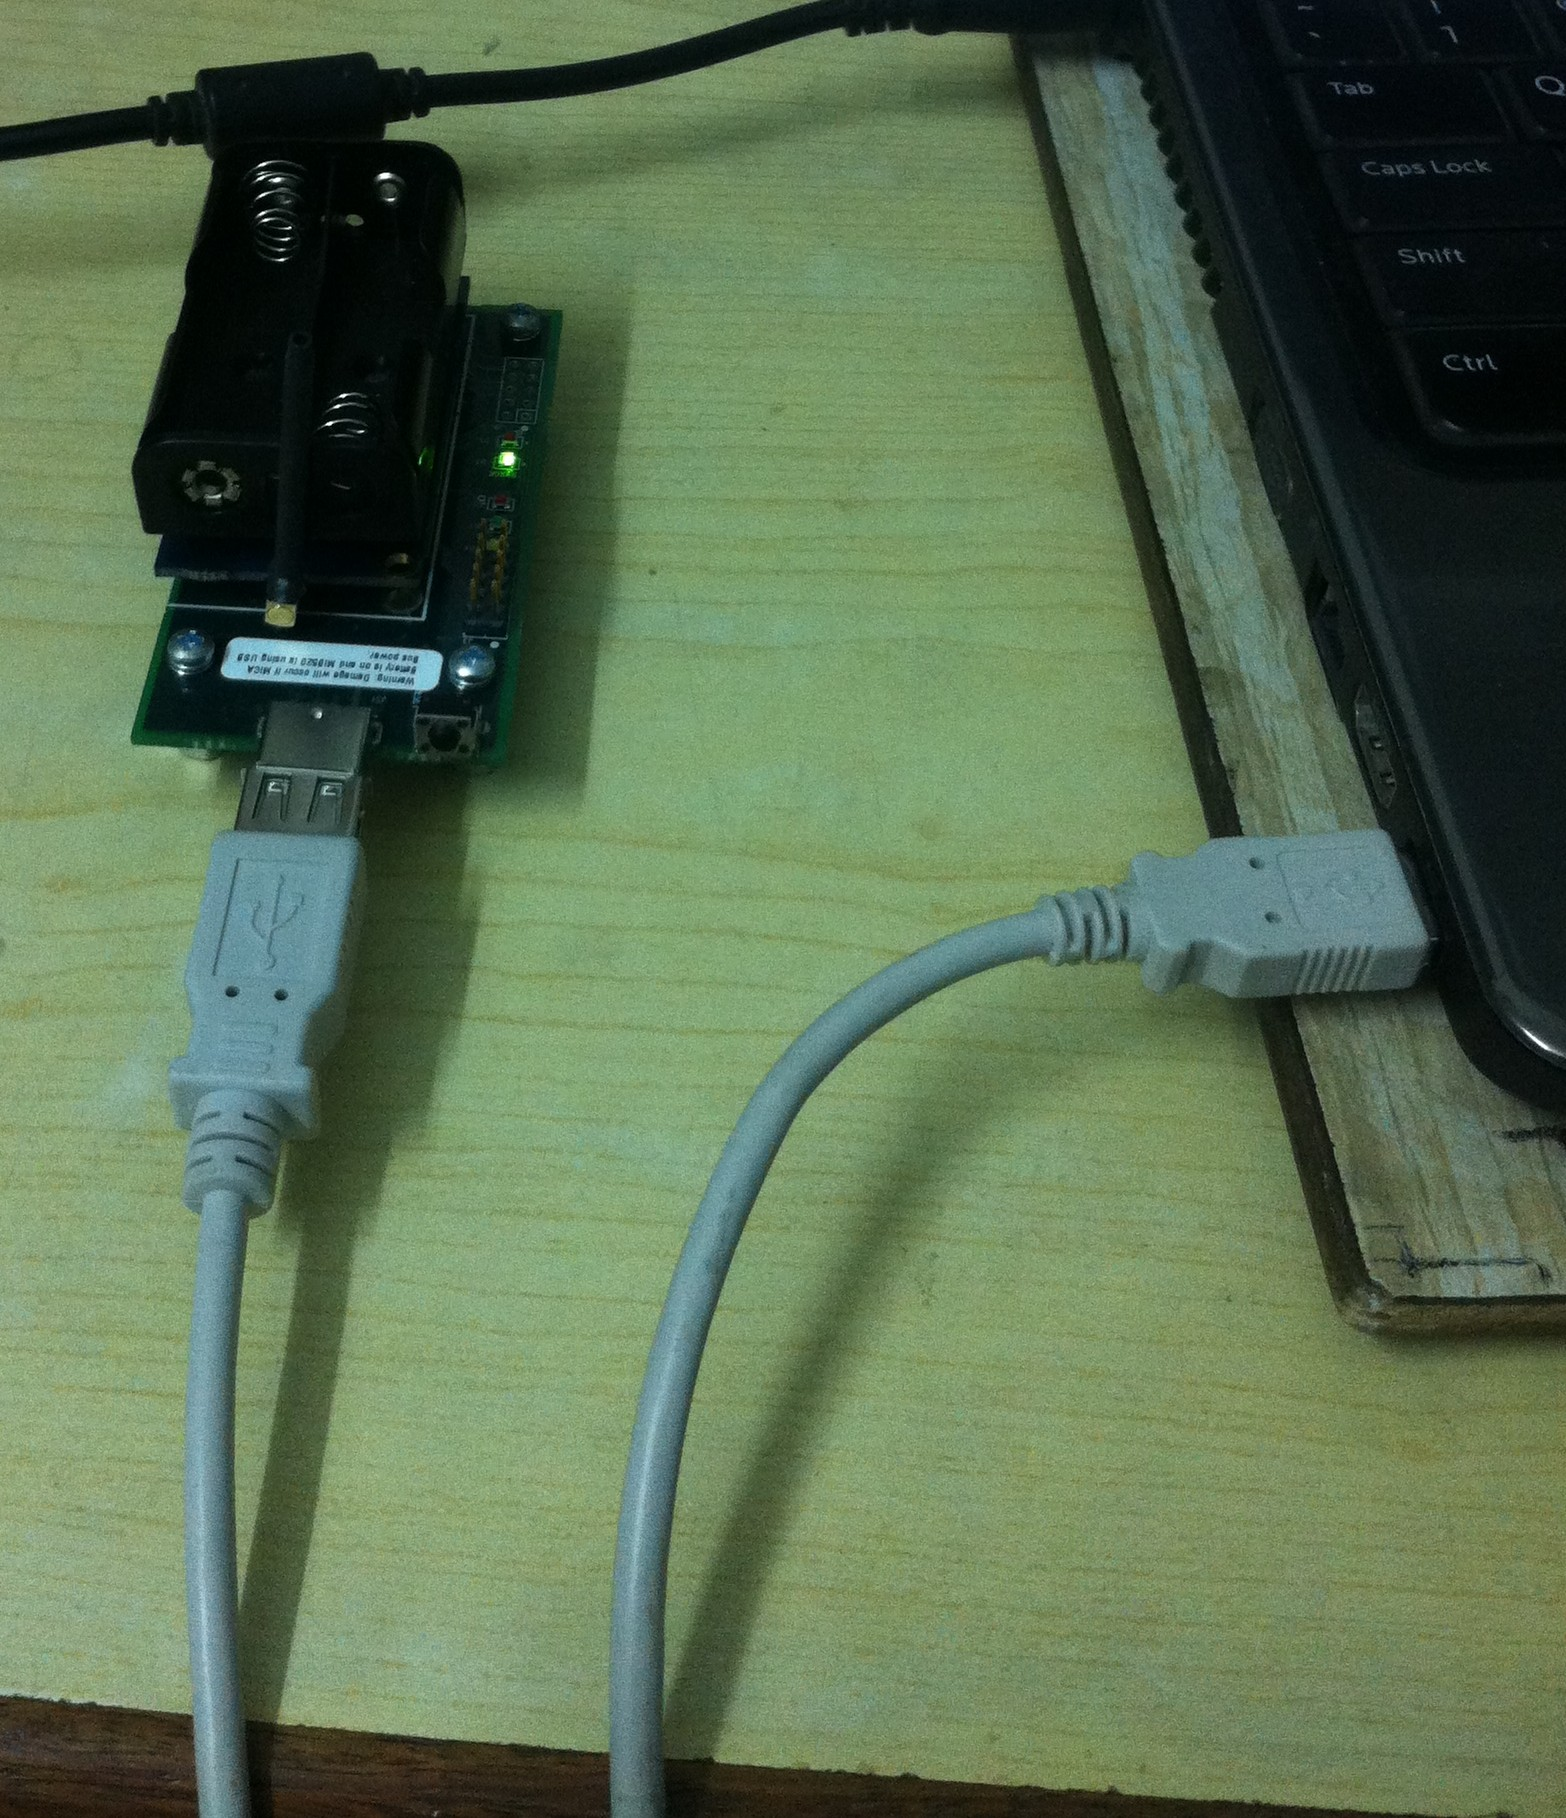
\includegraphics[scale=0.15]{images/18.JPG}
\caption{Base Station}
\label{bs}
\end{center}
\end{figure}

This mote interface board is used to program each mote via USB port. The mote attached to board runs on USB bus power and no external power supply is needed. This board offers two different ports, one for in-system programming and other for data transfer.

In our application we attach an IRIS mote having node id 0 (base station) to one of this board. The mote passes all packet it receives through radio to UART interface and vice versa. This board works as mediator between wireless network and our base station program. 

\subsection{TinyOS}
TinyOS is a free, open-source opertaing system which target low-powered wireless sensor netowork motes. It it totally written in nesC. TinyOS started as a collaboration between the University of California, Berkeley in co-operation with Intel Research and Crossbow Technology.

\vspace{0.5cm}
\begin{figure}[!h]
\begin{center}

\includegraphics[scale=0.5]{images/19.jpg}
\caption{TinyOS Logo}
\label{tinyos}
\end{center}
\end{figure}

The applications for TinyOS are written in nesC, which is optimized C language for sensor motes. Throughtout our system we have used TinyOS version 2.1.1.

\subsection{nesC: TinyOS Programming Language}
nesC (network embedded systems C), is a  and event-driven, component-based programming language. nesC is used to develop applications for TinyOS platforms. nesC is basically an extension to C programming language having different components which are wired together to perform one particular task.

The whole TinyOS has been implemented in nesC. nesC has completely different linking model than of C, the major challenge or problem does not lies in writing a piece of code, it is rather in combining these pieces together and make them work. nesC programs are built on components which are connected togather by carious interfaces.

In our system we have used nesC to program all IRIS motes which runs TinyOS. We have used many of already implemented modules and designed some of our own modules to make system work the way which we wanted.

\subsection{MIG (Message Interface Generator)}
MIG is a tool to generate code that process TinyOS messages. This tool generates a java class to encode or decode a TinyOS packet, basing itself on the net.tinyos.message infrastructure.

In our application this tool was useful at time of connecting base station: java application and IRIS mote with interface board which works as node id: 0.

\subsection{Java}
Java is general-purpose, object oriented programming language. We have used Java in our system to design GUI or front-end. End user can query through GUI designed (see figure \ref{gui}) and get results.

MIG tool is being used to create and interpret the received packets by our base station. We are using java swing feature to design the GUI. We are also using inbuilt \emph{HashMap} to apply hashing at BS which store the location of push items.

\section{System Modules}

In this section, we will look at implementation details of each and every module present in system. We will look at what they do, what are the structures that they use, the brief algorithm and lastly the connection diagram for each module. Starting from the lowest layer in hierarchy we have (i) Push Tags, (ii) Pull Tags, (iii) Mediator and, (iv) Base station. Let's start with the first one.

\subsection{Tags (Push Approach)}

These tags will be attached to the items which are required in emergency or instantly. These tags will keep pushing their details to upper layer periodically. Base station would maintain a local database about current location of all these items and update them as items change their positions. 

Tags will periodically broadcasts their presence using a structure defined below. This broadcasted packets will be received by the mediators of that region. These mediators will than make an array of such items and pass it to BS.

\begin{framed}
typedef nx\_struct PushTag

\{

\hspace{2em} nx\_uint16\_t node\_id; \hspace*{2em} \textit{own node id}

\}PushTag;
\end{framed}

The node id is its own node's own id by which it will be sought. These tags will not do anything on receiving packets, they will just keep broadcasting a packet having this structure in it.

Let's look at the algorithm they implement.
\begin{framed}
\begin{enumerate}
\item \textit{Add own node id to the structure `PushTag'.}
\item \textit{Broadcast packet containing that structure.}
\item \textit{Wait for specified period and, go to Step 1.}
\end{enumerate}
\end{framed}

This tag uses \emph{Timer} module to transmit packet at specific intervals. This module does not have any receive method. The connection diagram for PushTags is shown in figure \ref{push_dia}


\vspace{0.5cm}
\begin{figure}[!h]
\begin{center}
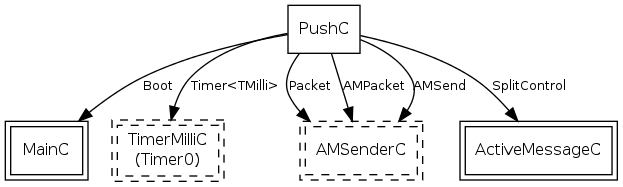
\includegraphics[scale=0.7]{images/20.png}
\caption{Connection Diagram for Push Tags}
\label{push_dia}
\end{center}
\end{figure}

As we have said this module just used Timer module, and a sender module to transmit data periodically.

\subsection{Tags (Pull Approach)}

Pull tags are used to tag the items which are relatively static in nature. We assume that at time of querying these items user can wait for some seconds. 

Unlike push tags pull tags will not transmit any packet periodically, which makes them energy efficient. Whenever this motes receives a packet it will first check weather it is a user request packet or not. If it is a user request packet then it will check weather required node id matches to its own node id or not. If node id matches then it replies to mediator indicating that user is looking for itself, otherwise it just ignores the packet and goes back to sleep. PullTag uses following structure to pass data from BS to tags.

\begin{framed}
typedef nx\_struct PullMsg

\{

  \hspace{2em}nx\_uint16\_t requiredid;	\hspace*{1em}	\emph{node id to be searched}

  \hspace{2em}nx\_uint16\_t mediatorid;	\hspace*{1em}\emph{node id of mediator under which sought node will be found.}

  \hspace{2em}nx\_uint16\_t flag;		\hspace*{4em}	\emph{0 - for pull request, 1- for pull reply.}

\} PullMsg;
\end{framed}

In the structure requiredid field is used to indicate user is looking for that particular item. Mediatorid is used to indicate the location of required node. So in case when query is being sent to all tags it is empty. That field is being filled once item user is looking for is found. And lastly the flag field is used to differentiate between this user request and reply. Again this flag is inverted by the tag which is sought.

Brief working/algorithm of pull tag is shown below.
\begin{framed}
\begin{enumerate}
\item \textit{Wait for incoming packet having `PullMsg' strcture in it.}
\item \textit{If (`requiredid' == own node id)}

\hspace*{2em}\textit{Mark `flag' = 1, set `mediatorid' = source node id and send packet back.}
\\
\textit{else}
\\
\hspace*{2em}\textit{Just ignore the packet, and go to step 1.}
\end{enumerate}
\end{framed}

So as we have just described in case of pull item search, base station would broadcast a query with structure shown above with requiredid entered by user and flag set to 0. Now when it reaches to all tags one of all tags' node id matches to required and then that node fills details about mediator id. Finally it again transmits that packet back to mediator which will forward reply to base station. Connection diagram for pull tag is shown in figure \ref{pull_dia}

\vspace{0.5cm}
\begin{figure}[!h]
\begin{center}
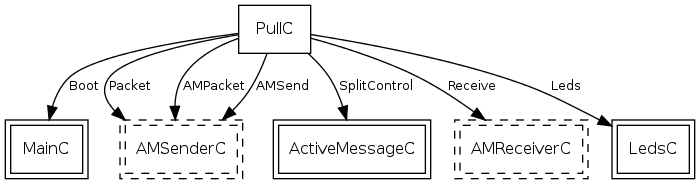
\includegraphics[scale=0.7]{images/21.png}
\caption{Connection Diagram for Pull Tags}
\label{pull_dia}
\end{center}
\end{figure}

The pull tags use two modules, one for receving the packets to receive user request and a sender module to reply.

\subsection{Mediators}

Mediators are the heart of our searching system, they are used to identify where actually the item is. As we have defined above due to high range problem of IRIS motes we have eliminated one level or mediators in implementation part.

Mediators have to do many tasks one of them if to pass aggregated data about push tags in its range to BS. Second is to implement data aggregation algorithm and forward packets according to that condition. And third is to pass user request and reply packets for pull tags at time of query.

It uses following structure to pass details about push tags to BS.

\begin{framed}
typedef nx\_struct AggregationMsg

\{

  \hspace{2em}nx\_uint16\_t nodeid;\hspace*{3em}	\emph{Mediator node id.}

  \hspace{2em}nx\_uint16\_t size;\hspace*{4em}	\emph{Number of nodes under that mediator.}

  \hspace{2em}nx\_uint16\_t nodes[10];\hspace*{2em}	\emph{Node ids of the items}

\} AggregationMsg;
\end{framed}

Here nodeid is its own node id, size is the array size till what array has been filled and nodes[ ] array stored the node id of various items that currently reside in it's region. So when base station gets one of this packet it updates database entry of the node ids specified in array to \emph{nodeid} field as that all items are now under this mediator's range.

Mediators in our system implements following algorithm.

\begin{framed}
\begin{enumerate}
\item \textit{Wait for incoming message.}
\item\textit{Check the structure contained in packet.}\\
\hspace*{1em}\textit{If it's `PushTag', add node id to local array.}\\
\hspace*{1em}\textit{If it's `PullTag', Using flag field check weather it is user request or reply.}\\
\hspace*{3em}\textit{If it is a user request the broadcast it to all tags.}\\
\hspace*{3em}\textit{If it is reply then pass it to base station.}\\
\hspace*{1em}\textit{If it's `AggregationMsg', then decide according to the ``Data Aggregation" algo. }
\item \textit{Prepare and forward a packet containing `AggregationMsg' structure periodically to inform base station about items in its region.}
\end{enumerate}
\end{framed}

As we have said mediators have to listen from many different sources so, our implantation uses more than on instance of AMReceive module (see figure \ref{mediator_dia}). Other than that as more than one methods use AMSend to send packets and we have single transmitter on mote, we have to take care about concurrent radio use.

\vspace{0.5cm}
\begin{figure}[!h]
\begin{center}
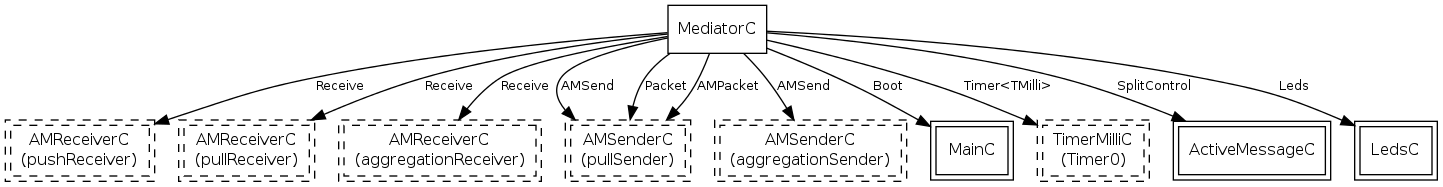
\includegraphics[scale=0.35]{images/22.png}
\caption{Connection Diagram for Mediators}
\label{mediator_dia}
\end{center}
\end{figure}

As show in figure, in the mediators we are using three different instance of receive modules to receive, two different sender modules to transmit different packets and a timer module periodically infrom BS about push tags in its range.

\subsection{Base Station}
Base station is the sink of network. End user will interact with base station only to query an item and get results. We have two major module in base station, first is IRIS mote + interface board which is used to forward packets received using radio to our java application. Second is java application which is used to provide easy-to-use interface to end users through which they can use our system. 

The IRIS mote attached to interface board implements a simple program which just pass all packets received via radio interface to UART and pass packets received via UART to radio interface. The java application prepares a packet at time of user query for pull tag and broadcasts it. We are using \emph{mig} tool defined above to interpret TinyOS packets.

Basic working of BS are as shown below.

\begin{framed}
\begin{enumerate}
\item \textit{Case 1: User queries for some item:}\\
\hspace*{1.5em}\textit{If it is an item using `Push Approach', show location from local database.}\\
\hspace*{1.5em}\textit{If it is an item using `Pull Approach', prepare a user request packet and broadcast it.}
\item \textit{Case 2: System receives a packet:}\\
\hspace*{1.5em}\textit{If it is an data aggregation message just update the local database.}\\
\hspace*{1.5em}\textit{If incoming packet is reply of previously sent user request containing `PullTag', show results through GUI.}
\end{enumerate}
\end{framed}

We have used hashing to store the locations about push tags on base staion. To find any item user first has to query using the node id, and system will show results using a preloaded picture of locality where that item currently resides (see figure \ref{ex}).


\vspace{0.5cm}
\begin{figure}[!h]
\begin{center}
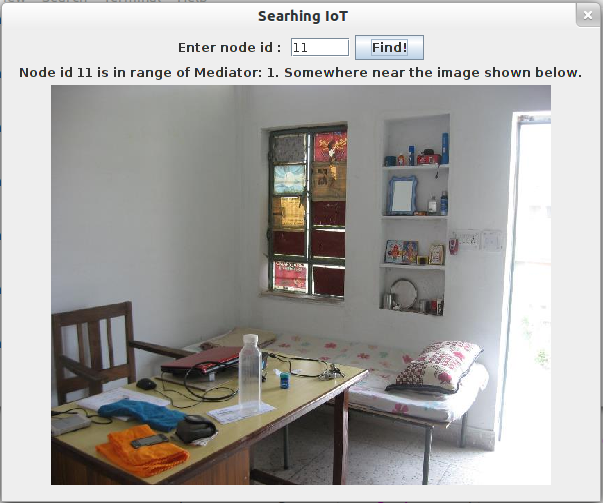
\includegraphics[scale=0.55]{images/16.png}
\caption{Base station GUI}
\label{ex}
\end{center}
\end{figure}

\section{Experimental Results}
In this section we are going to look at the experimental setup details and some results that we have got. To varify our system's working, we have prepared a prototype of it.

We have covered three different places, two rooms and a corridor. Our system will tell where the required item currently is, with a preloaded image of that place. We are considering the most important parameters for searching like \emph{response time, accuracy} and \emph{effectiveness}. Let's look at each of them in detail.

\begin{itemize}
\item \textbf{Response Time:} This is the most important parameter of our search, as user wants results immediately. For the push tags results will be instant as base station will already be having their location details, so user has to wait only for querying pull items. After performing various experiments we have observed that our system takes mearly 1-2 seconds to find a location of any item.
\item \textbf{Accuracy:} This is also important feature as, if results are not accurate they are of no use because user wont be able to find that item! In our experiments we have found that our system produces accurate results most of the time. There is a problem only when regions covered by mediators overlap. When an item is in range of two different mediators, system will show only one and that might not be the actual place where item is. To overcome this problem we have to make sure that regions do not overlap, and to go further we can use RSSI value to decide actual location when two or more mediator claims for same item.
\item \textbf{Effectiveness:} One can argue that let this system be fast and accurate, but weather it is actually effective than manual search? According to \cite{13} it takes minimum 10s and at max 300s to search any item manually, while as we just said our system takes few seconds to do the same.
\end{itemize}

We also have to consider various things like number of tags, if we increase items in home weather our system will produce the same results or not. We can say that our proposed hybrid approach takes care of this issue as most of the items will use pull approach, so it will not create any extra overhead on network or on base station database.

In this chapter we have seen various implementation details like tools and technologies used, we have also discussed working of each module in detail. At last we have seen our experimental setup and results we got. In next chapter we will finally concude our thesis and provide some future extention or ways in which one can extend this work.


\newpage
\chapter{CONCLUSIONS AND FUTURE WORKS}
\vspace{0.2cm}
In last chapter, we have discussed about implementing the whole system. In this chapter, we will finally conclude our thesis and provide some possible future direction to our work.

\section{Conclusions}
As we have said Internet of Things is \emph{the} future of current Internet. It is a vision to connect each real-world entity and given them web presence. In section 1.3 we have looked at various applications and ways in which IoT has potential to change the way we live our daily life.

Searching will be an important task in such environment as we misplace our items easily and then we waste our time in finding them. To provide a solution here we have developed a mechanism that can help you to find your lost item in your home/office. There are many exisiting techniques which does same thing but they all some problems associated with them like some uses centralized approach that makes them unable to scale, some requires more time to produce results, etc.

Our system requires minimal setup, user just has to tag all real-world entities once. We have described the layered architecture and various other algorithms about how system will work. Our system handles most of the major issues like scalability, real-time updates, quick results, user-friendliness with approached like aggregation algorithm, hybrid push-pull approach, hashing at server and instead of just specifying room name we are providing the actual image of that room.

After that we have discussed about each module's implementation details and the technologies used to implement that. We have also described the modules used and their interconnection using diagrams. At last we evaluated our system, based on various parameters. We can conclude that humans are powerful sensors, they just require an approximate location to find any item.

\section{Future Works}
Our system can be extended in various ways like, we can add some processing and memory to mediators. In that case mediators will also contain detail about tags in its range so we do not need to broadcast each query to each tag.

Our current system lacks feature of multiple-user query at a time, user can query only from base station. To resolve that user must be able to query from his smart phone or some other remote location at same time to our system. We also need to add privacy mechanism in such case as in our current system we can search only from base station, so there is no need for security in that case.

One more thing, we have to replce these IRIS motes which are used as tag with some cheap technology like RFID to make our system deployed widely.

In the end we can say that, our system has the potential to change the way people live their life everyday.

%%%%%%%%%%%%%%%%%%%%%%%%%%%%%
\newpage
\addcontentsline{toc}{chapter}{References}
%\markright{Bibliography}
\begin{thebibliography}{1000}
\vspace*{.5cm}

%1
\bibitem{1}
 Kevin Ashton, That `Internet of Things' Thing. {\em RFID Journal} 22: pp. 97-114, 2009.
\bibitem{2}
Agrawal S. and Das M.L., ``Internet of Things - A Paradigm Shift of Future Internet Applications''.{\em Nirma University International Conference on Current Trends In Technology Engineering (NUiCONE)} pp. 1-7, Ahmedabad, 2011.
\bibitem{image_roadmap}
``Technology Roadmap'' http://en.wikipedia.org/wiki/File:Internet\_of\_Things.png
\bibitem{image_cisco}
``IoT : Infographic'' http://blogs.cisco.com/news/the-internet-of-things-infographic/
\bibitem{3}
``Bicing'' http://www.bicing.cat/
\bibitem{4}
``WEMO'' http://www.belkin.com/wemo/
\bibitem{5}
``Nike+iPod'' http://www.apple.com/in/ipod/nike/
\bibitem{6}
``Botanicalls'' http://www.botanicalls.com/
\bibitem{7}
Das R. and Harrop P., ``RFID forecasts, players and opportunities 2011-2021'',{\em IDTechEx.com, Tech. report}, 2010.
\bibitem{8}
Sundmaeker H. and Guillemin P. and Friess P. and Woelffle S., ``Vision and challenges for realising the Internet of Things'', {\em CERP-IoT, European Commission}, pp. 72-73, Luxembourg, March 2010.
\bibitem{9}
Zhang D. and Yang L.T. and Huang H., ``Searching in Internet of Things: Vision and Challenges'', {\em IEEE 9th International Symposium on Parallel and Distributed Processing with Applications (ISPA), 2011}, pp.201-206, Busan, 2011.
\bibitem{10}
Anderson R., Security engineering: a guide to building dependable distributed systems.{\em Wiley Publications}, 2010.
\bibitem{11}
Wang H. and Tan C.C. and Li Q., ``Snoogle: A Search Engine for Pervasive Environments'', {\em IEEE Transactions on Parallel and Distributed Systems}, Vol. 21, No. 8, pp.1188-1202, August 2010.
\bibitem{12}
Tan C.C. and Sheng B. and Wang H. and Li Q., ``Microsearch: A Search Engine for Embedded Devices Used in Pervasive Computing'', {\em ACM Transactions on Embedded Computing Systems (TECS)}, Vol. 9, No. 4, pp. 1-29, New York, March 2010.
\bibitem{13}
Yap K.K. and Srinivasan V. and Motani M., ``Max: Human-Centric Search of the Physical World'', in {\em SenSys '05: Proceedings of the 3rd international conference on Embedded networked sensor systems}, ACM, pp. 166-179, San Diego, 2005.
\bibitem{14}
Frank C. and Bolliger P. and Mattern F. and Kellerer W., ``The Sensor Internet at Work: Locating Everyday Items Using Mobile Phones'', {\em Pervasive and Mobile Computing}, Elsevier ,Vol. 4, No. 3, pp. 421-447, 2008.
\bibitem{15}
Yan, T. and Ganesan, D. and Manmatha, R., ``Distributed Image Search in Camera Sensor Networks'' in {\em SenSys '08: Proceedings of the 6th ACM conference on Embedded network sensor systems}, ACM, pp. 155-168, 2008.
\bibitem{16}
Romer K. and Ostermaier B. and Mattern F. and Fahrmair M. and Kellerer W.,``Real-time search for real-world entities: A survey'', {\em Proceedings of IEEE}, Vol. 98, No. 11, pp. 1887-1902, Nov. 2010. 
\bibitem{17}
Ostermaier, B. and Elahi, B.M. and Romer, K. and Fahrmair, M. and Kellerer, W., ``Dyser: towards a real-time search engine for the web of things'' in {\em SenSys '08: Proceedings of the 6th ACM conference on Embedded network sensor systems}, ACM, pp. 429-430, 2008.
\bibitem{18}
Bapat, Tejas A., K. Selçuk Candan, V. Snehith Cherukuri, and Hari Sundaram. ``AURA: Enabling Attribute-based Spatial Search in RFID Rich Environments." in {\em ICDE'09. IEEE 25th International Conference on Data Engineering, 2009.}, pp. 1211-1214. IEEE, 2009.
\bibitem{19}
Jianwei Liu; Haiying Shen; Ze Li; Loeb, S.; Moyer, S.; , ``SCPS: A Social-Aware Distributed Cyber-Physical Human-Centric Search Engine," {\em Global Telecommunications Conference (GLOBECOM 2011), 2011 IEEE} , vol., no., pp.1-5, 5-9 Dec. 2011
\bibitem{20}
Stankovic, John A. ``Wireless sensor networks." {\em computer 41, no. 10} (2008): 92-95.
\bibitem{21}
Ravindranath, Lenin, Venkata N. Padmanabhan, and Piyush Agrawal. ``Sixthsense: RFID-based enterprise intelligence." in {\em Proceedings of the 6th international conference on Mobile systems, applications and services,} pp. 253-266. ACM, 2008.
\bibitem{22}
Christophe, Benoit, Vincent Verdot, and Vincent Toubiana. ``Searching the'Web of
Things'." in {\em Fifth IEEE International Conference on Semantic Computing (ICSC),2011}, pp. 308-315. IEEE, 2011.
\bibitem{23}
Ding, Zhiming; Dai, Jian; Gao, Xu; Yang, Qi; , ``A Hybrid Search Engine Framework for the Internet of Things," {\em Web Information Systems and Applications Conference (WISA), 2012 Ninth} , vol., no., pp.57-60, 16-18 Nov. 2012
\bibitem{24}
Jin, Xin, Daqiang Zhang, Qin Zou, Genlin Ji, and Xiaojun Qian. ``Where searching will go in Internet of Things?." In {\em Wireless Days (WD), 2011 IFIP,} pp. 1-3. IEEE, 2011.


\end{thebibliography}
%----------------------------------------------------------------------------
\end{document}